\documentclass{article}
\usepackage{proj1}
\usepackage{natbib}
\usepackage{fancyhdr}  %headers and footers
\usepackage{subcaption}
\usepackage{caption}
\usepackage{graphicx}
%set spacing between lines (DO NOT CHANGE SPACING)
\linespread{1.25} %normally 1.25
\setlength{\parindent}{0cm}
\graphicspath{{Images/}}
%\underline{\smash{\beta}} makes underlining at the same distance

\usepackage{hyperref}


\hypersetup{
	colorlinks,
	allcolors=.,
	urlcolor=blue,
}
\usepackage{color}
\urlstyle{same}
%Definition of margins (DO NOT ALTER!)+

%\usepackage[a4paper, top=1in, left=1.0in, right=1.0in, bottom=1in, includehead, includefoot]{geometry} %Usually have top as 1in

%%%%%%%%%%%%%%%%%%%%%%%%%%%%%%%%%%%%%%%%%
% +++ ... +++ denotes something to be changed
%%%%%%%%%%%%%%%%%%%%%%%%%%%%%%%%%%%%%%%%%%
%Commands
\newcommand{\PDEsmall}[2]{\frac{\partial #1}{\partial #2}}
\newcommand{\PDE}[2]{\dfrac{\partial #1}{\partial #2}}
\newcommand{\folds}{(x_0,y_0)}
\newcommand{\st}{such that }
\newcommand{\wrt}{with respect to }
\newcommand{\vdp}{Van der Pol }
\newcommand{\wlg}{without loss of generality }
\newcommand{\Wlg}{Without loss of generality }
%%%%%%%%%%%%%%%%%%%%
\title{Fast Slow Dynamics - the van der Pol Oscillator}
\author{}
\date{October 2018}

\pagenumbering{Roman} % Start roman numbering

\begin{document}

\maketitle
\newpage

\tableofcontents
\newpage
\listoffigures

%\listoftables
\newpage
%\lstlistoflistings%\lstlistlistingname
%\newpage
\pagenumbering{arabic} % Switch to normal numbers
\pagestyle{fancy}

\begin{abstract}
	This project will be considering the Fast-Slow dynamics in non-linear ordinary differential equations. The project will start by considering the theory associated with Fast-Slow dynamical systems such as Geometric Perturbation Theory (Section \ref{GSPT}). Then the project moves onto two-dimensional systems by first looking at the general form, using \citet{krupa2001} theory (Section \ref{Intro}), before applying it to the \vdp system (Section \ref{sec:the-van-der-pol-equation}). From here the project will also consider the non-hyperbolicity of the fold points present in the system, where a jump might occur (Section \ref{sec: VDP Blowup}). Once the system has been `blown-up' for the normal case, it is prudent to consider the canard system - where the parameter $ \lambda $ is introduced. This could cause a split within the manifolds or a Hopf bifuraction could occur causing a periodic solution (Sections \ref{sec:canard-points} and \ref{sec:separation-of-the-manifolds}). Once this has been considered, the next step is to consider the Fast-Slow system in a three dimensional case for folded singularities (Section \ref{sec:folded-singularities-in-a-three-dimensional-system}) before continuing onto the theory behind Mixed Mode Oscillations (Section \ref{sec: MMO Oscilaltions}). \textbf{Lastly, the project will discuss the numerical simulations associated with the construction of the models and the results obtained (Section \ref{sec:matlab-stuff}}).
\end{abstract}



\section{MATLAB Stuff}\label{sec:matlab-stuff}
\input{Chapters/MATLAB.tex}

\section{Fast-Slow Systems}\label{Intro}


\section{Fast-Slow Systems}\label{Intro}
Fast- Slow systems are systems of differential equations that can be viewed on two different time scales, which are separated by a parameter.
These systems are generally of the form
\begin{align} \label{FastS}
\begin{cases}
x' &=\frac{dx}{dt}= f(x,y,\lambda, \epsilon)\\
y' &= \frac{dy}{dt}= \epsilon g( x,y, \lambda, \epsilon),
\end{cases}
\end{align}
which is called the fast system.
Using a change of variables, $t = \frac{\tau}{\epsilon} $ this can be rewritten as
\begin{align}
\begin{cases}
\epsilon \dot{x} &= \epsilon \frac{dx}{d \tau} = f(x,y,\lambda, \epsilon)\\
\dot{y} & = \frac{dy}{d \tau} =  g( x,y, \lambda, \epsilon),
\end{cases}\label{SlowS}
\end{align}
called the slow system.

Here $x$ is called the fast variable, while $y$ is the slow variable. $\lambda$ is a parameter, $\epsilon$ is the time scale separation parameter and satisfies $0< \epsilon << 1$. The functions $f$ and $g$ are required to be sufficiently smooth ( depending on literature $C^1, C^\infty, C^{r+1} for C^r$ invariant manifolds. Choose later, maybe $C^r$ considering fenichel theorem)
It is generally possible to have three or more time scales, separated by additional time scale separation parameters parameters, as well as more state-space variables. 

In order to analyse systems (\ref{FastS}) and (\ref{SlowS}) using Geometric Singular Pertubation Theory (GSPT), the singular limit $\epsilon \to 0$ is considered:

\begin{align} \label{FastS0}
\begin{cases}
x' &=\frac{dx}{dt}= f(x,y,\lambda, \epsilon)\\
y' &= 0,
\end{cases}
\end{align}
which is called the layer problem and
\begin{align}\label{SlowS0}
\begin{cases}
0 &= \epsilon \frac{dx}{d \tau} = f(x,y,\lambda, 0)\\
\dot{y} & = \frac{dy}{d \tau} =  g( x,y, \lambda,0),
\end{cases}
\end{align}
called the reduced system.

Considering (\ref{SlowS0}), the first equation is $f(x,y,\lambda, 0)=0$ and a manifold can be defined as:
\begin{align} \label{CriticalS}
S= \left\{ (x,y) : f(x,y,\lambda, 0)=0 \right \},
\end{align}
called the critical manifold, where, by definition of $S$, the points $(x,y) \in S$ are equilibria of (\ref{FastS0}). Before we continue, it is useful to have a visual interpretation of these flows, 
\begin{figure}[h!]\centering
	%\includegraphics{./}
%	\caption{Flows in our \vdp system.}
	\label{fig: vdp flow diagram}
\end{figure}
where we can see that the flows will travel towards our fold point, following the relevant branches.
\section{Geometric Singular Pertubation Theory} \label{GSPT}

The main idea of GSPT is the following: Under certain conditions it can be concluded that the critical manifold $S=S_0$, where $\epsilon \to 0$ persists as an invariant manifold $S_{\epsilon}$ under a small pertubation $\epsilon >0$, if $\epsilon$ is sufficiently small. 
(In higher than 2 dimensions the idea of transversality of the flow of the stable and unstable manifolds is essential for analysis, while in 2 dimensions this is rather trivial.)
The main contribution to GSPT comes from Fenichel Theory and his three Theorems can be summed up in one, according to ( reference MMO Paper or book).
However, before stating the Theorem, some formal definitions are needed.

\begin{definition}{\textbf{Normal Hyperbolicity}} \label{NormHyp}
	\\
	A submanifold $M \subseteq S$ is called normally hyperbolic, if the Jacobian $ \frac{\partial f}{\partial x}(x,y, \lambda, 0),$ where $(x,y) \in M$, has only eigenvalues with nonzero real part.
\end{definition} (reference paper 1)

Moreover, the points $(x,y) \in M$, $M$ normally hyperbolic, are hyperbolic equilibria of (\ref{FastS0}). (ref:MMO)
A normally hyperbolic submanifold can be classified according to its stability property: If $M$ has only eigenvalues with positive real part it is called repelling, if $M$ has only eigenvalues with negative real part it is called attracting and if $M$ is neither attracting nor repelling it is called a saddle-type submanifold. (ref:MMO paper) \\
Furthermore, stable and unstable manifolds can be defined as $W^s(M)$  and $W^u(M)$, corresponding to the eigenvalues with negative and positive real part, respectively.
(???? pretty sure there are two different concepts in the last two sentences.. check needed)
Furthermore, with the following definition it is established which notion of distance is going to be employed throughout this analysis.

\begin{definition}{\textbf{Hausdorff Distance}}\\
	The Hausdorff Distance of two nonempty sets $V,W \subset \mathbf{R}^n$, for some $n \in \mathbf{N}$ 
	is defined as 
	\begin{align*}
	d_H(V,W)= \max \{ \sup_{v \in V} \inf_{w \in W} || v- w ||, \sup_ {w \in W}\inf_{v \in V} || v- w ||\}.
	\end{align*}
	(ref: book kuehn)
\end{definition}

Now Fenichel's Theorem can be stated:
\begin{theorem}{\textbf{Fenichel's Theorem}} \label{Fenichel}
	\\
	Suppose $M=M_0$ is a compact, normally hyperbolic submanifold  (possibly with boundary) of the critical manifold $S$ (\ref{CriticalS}) and  that $f, g \in C^r, r < \infty $. Then for $\epsilon >0$, sufficiently small, the following hold:\\
	(F1) There exists a locally invariant manifold $M_{\epsilon}$, diffeomorphic to  $M_0$. Local invariance means that $M_{\epsilon}$ can have boundaries through which trajectories enter or leave.\\
	(F2) $M_{\epsilon}$ has a Hausdorff distance of $O(\epsilon)$ from $M_0$.\\
	(F3) The flow on $M_{\epsilon}$  converges to the slow flow as $\epsilon \to 0$.\\
	(F4) $M_{\epsilon}$ is $C^r$- smooth.\\
	(F5) $M_{\epsilon}$ is normally hyperbolic and has the same stability properties with respect to the fast variabes as $M_0$ (attracting, repelling or saddle type).\\
	(F6) $M_{\epsilon}$ is usually not unique. In regions that remain at a fixed distance from the boundary of  $M_{\epsilon}$, all manifolds satisfying (F1)-(F5) lie at a Hausdorff distance $O(e^{-K/\epsilon})$ from each other for some $K>0$ with $K=O(1)$.\\
	The normally hyperbolic manifold $M_0$ has associated local stable and unstable manifolds
	\begin{align*}
	W^s(M_0) =\cup_{p \in M_0} W^s(p) \textrm{\ \ and\ \ } W^u(M_0) =\cup_{p \in M_0} W^u(p),
	\end{align*}
	where  $W^s(p)$ and $W^u(p)$ are the local stable and unstable manifolds of $p$ as a hyperbolic equilibrium of the layer equations, respectively. These manifolds also persist for $\epsilon > 0$, sufficiently small: there exist locally stable and unstable manifolds $W^s(M_\epsilon)$ and $W^u(M_\epsilon)$, respectviely, for which conclusions (F1) - (F6) hold if we replace $M_\epsilon$ and $M_0$ by  $W^s(M_\epsilon)$ and $W^s(M_0)$ (or similarly by  $W^u(M_\epsilon)$ and $W^u(M_0)$).
\end{theorem} +++direct citation needed for theorem (MMO) +++

Fenichel's Theorem establishes that the submanifold $M_0$ of the critical manifold $S_0$ persists as slow manifold $M_\epsilon$ as $\epsilon >0$, given it is compact and normally hyperbolic. The theorem furthermore establishes that the stable and unstable manifolds persist as well as the individual fibres of these manifolds, namely $W^s(p)$ and $W^u(p)$, that are associated to each base point $p \in M_0$.
Therefore, under the assumptions of the theorem, the flow of the fast-slow system (\ref{FastS})/(\ref{SlowS}) remains $O(\epsilon)$ close to the flow of the system (\ref{FastS0})/(\ref{SlowS0}) in the singular limit $\epsilon \to 0$.
\\
The importance of this result lies in the fact that the behaviour of the full system can be analysed by looking at the system in the singular limit instead, which is often more practical.


++++++++++++also trajectories can be constructed and tested using fenichel... paper 1++++++++++




\section{Singularities and Fold Points}\label{sec:singularitiesandfoldpoints}
One of the requirements of Fenichel's Theorem is normal hyperbolicity \citep{Kuehn}. However, Fast-Slow systems can display singular points where normal hyperbolicity is no longer given and therefore the conclusions of Theorem \ref{Fenichel} no longer hold at these singularities - where trajectories can jump between fast and slow flow. The singularities in the setting of Fast-Slow systems are points $(x_0,y_0)$ on the critical manifold $S_0$, for which the Jacobian ($ J \ \text{at} \ {\partial x}(x_0,y_0, \lambda, 0)$) has one or more eigenvalue with zero real part. Comparing this with Definition \ref{NormHyp} shows that this is a negation of normal hyperbolicity. The simplest of those singularities are called a fold point, which is defined as follows:
\begin{definition}{\textbf{Fold Point}} \label{FoldDef} \\
	A fold point $(x_0,y_0) \in S_0$ is a point where the Jacobian $ \frac{\partial f}{\partial x}(x_0,y_0, \lambda, 0)$ has only one eigenvalue with zero real part.
\end{definition}
%At the fold point, the system (Equation \ref{FastS0}) undergoes a saddle-node bifurcation. (+++explain?++++)
Moreover we say that the fold point is non-degenerate if it satisfies the non-degeneracy assumptions,
\begin{align} \label{NonDeg}
\begin{cases}
\frac{ \partial ^2 f}{ \partial x^2} (x_0,y_0, \lambda, 0) \neq 0, \\
\frac{\partial f}{\partial y}(x_0,y_0, \lambda, 0) \neq 0.
\end{cases}
\end{align}
Furthermore, if $(x_0,y_0)$ satisfies the transversality condition $g(x_0,y_0, \lambda, 0) \neq 0$, then it is called a generic fold point.
For these generic folds there exists a theorem that states that the slow flow on $S_\epsilon$ near $(x_0,y_0)$ has either positive or negative sign, implying that no equilibria of the slow flow are close to $(x_0,y_0)$. Therefore, for generic fold points no canards will be observed, which is a relevant observation for Section \ref{sec:canard-points}. First, we must find the fold points in the system.\\
\subsection{Fold Points in the Van der Pol System }
Considering the manifold $S= \{ (x,y) : 0=y-\frac{x^3}{3}+x^2:=f \}$, the Jacobian $\pd{f}{x}(x,y,0) = 2x-x^2 $, which has eigenvalues with zero real part at $x^{1,2}_0= 0,2$ -- together with the corresponding $y^{1,2}_0$ are singularities of the system.
Further analysis has to be done below in order to conclude that they are generic fold points.
The points of interest are $(x_0^1,y_0^1)=(0,0)$ and $(x_0^2,y_0^2)=\left(2,\dfrac{4}{3}\right)$. By Definition \ref{FoldDef}, there is only one eigenvalue with zero real part at $(x_0,y_0)$. Evaluating the Jacobian at each of the points in turn shows:
\begin{align*}
\begin{cases}
\frac{ \partial f}{\partial x}(x_0^1,y_0^1,0) =0 \\
\frac{ \partial f}{\partial x}(x_0^2,y_0^2,0) =0,
\end{cases}
\end{align*}
where each of the zeros are simple.
Therefore $(x_0^1,y_0^1)$ and $(x_0^2,y_0^2)$ are fold points.
These points are nondegenerate if the non-degeneracy assumptions (Equation \ref{NonDeg}) hold:
\begin{align*}
\begin{cases}
\frac{ \partial ^2 f}{ \partial x^2} (x_0^1,y_0^1, 0) = 2-2 x_0^+ = 2 \neq 0 \\
\frac{\partial f}{\partial y}(x_0^1,y_0^1, 0) = -1 \neq 0,
\end{cases}
\end{align*}
and equivalently for the other fold point
\begin{align*}
\begin{cases}
\frac{ \partial ^2 f}{ \partial x^2} (x_0^2,y_0^2,0) = -2 x_0^2 =4\neq 0 \\
\frac{\partial f}{\partial y}(x_0^2,y_0^2, 0) = -1 \neq 0.
\end{cases}
\end{align*}
Therefore, the two fold points are non-degenerate.
Futhermore, it can be checked if a fold point is generic. It then has to satisfy the transversality condition $g(x_0,y_0,0) \neq 0$.
The two fold points considered here are generic, since 
\begin{align*}
g(x_0^1,y_0^1,0)= -1\neq 0 \\
g(x_0^2,y_0^2,0)= 1 \neq 0.
\end{align*}

We know that normal hyperbolicity of the Van der Pol system breaks down at the fold points. Fenichel Theory can be applied for regions that are not in the neighbourhood of the fold points. However, a different approach has to be employed for the analysis of the dynamics around the folds. We need to use a new method called the Blow Up Method, which is discussed in Section \ref{sec: VDP Blowup}.\\

Systems containing non-generic folds or other types of singularities can display different types of periodic orbits.
\subsubsection{Extended System} \label{sec: extended sys blowup}
The canonical system (Equation \ref{eq: canonical}) is then extended to three dimensions by considering $\epsilon'=0$. 
\begin{equation} \label{extended FS}
\begin{aligned}
&x'=-y+x^2+h(x) \\
&y'=\epsilon(x-1)\\
&\epsilon'=0.
\end{aligned}
\end{equation}


Analysing the stability of the three dimensional system, three eigenvalues can be found by considering the Jacobian matrix, in the singular limit $\epsilon=0$: 
\begin{equation} 
J=\begin{vmatrix} 2x-x^2 & -1&0 \\ 0 & 0&0\\0&0&0\end{vmatrix}
\label{eq: Eigenvalues}
\end{equation}
This is an upper triangular matrix and hence $(\lambda_1.\lambda_2,\lambda_3)=tr(J)= (2x-x^2,0,0)$. Therefore, at the fold points, where $x=0$ or $x=2$, $\lambda_i=0 \ \text{for} \ i=1,2,3$, there exists a zero eigenvalue on $S$. Note that at these points $S$ is not normally hyperbolic.
The critical manifold has to be divided as follows:
\begin{align*}
S^a &=\bigg \lbrace (x,y): y = x^2-\frac{x^3}{3}, x< 0 \bigg \rbrace \cup \bigg \lbrace (x,y): y = x^2-\frac{x^3}{3}, x>2 \bigg\rbrace \\
S^r &= \bigg\lbrace (x,y): y = x^2-\frac{x^3}{3}, 0< x< 2 \bigg\rbrace,
\end{align*}
such that $S^a \cup S^r \cup \{0\} \cup \{2\} = S$.
The manifolds $S^a_0$ and $S^r_0$ are normally hyperbolic everywhere and  Theorem \ref{Fenichel} (Fenichel's) can be applied in order to conclude the persistence of the manifold as slow manifolds $S^a_\epsilon$ and $S^r_\epsilon$. At the points $x=0$ and $x=2$ the normal hyperbolicity is not given, since the eigenvalue associated to $S$ is zero at these points.
%++++++Note: technically the paper mentions here the centre manifold M, stressing the three dimensionality of the problem. if we want that it can be added+++++++++
\\
\\
In the analysis of the reduced system it became apparent that the fold points are singularities of the reduced flow on $S_0$, and therefore the dynamics in the singular limit cannot be determined. Furthermore, Fenichel Theory does not apply at the folds because normal hyperbolicity breaks down at these points, as discussed above. Therefore, even if the dynamics around the folds in the singular limit were known, no conclusions could be drawn for the perturbed system with $S_\epsilon$.
Alternative methods have to be employed to describe the dynamics on the fold points in the singular limit and furthermore to be able to conclude the dynamics of the full system at the fold points from this analysis.
The method considered for analysis is called the Blow-Up Method.




\section{The Van Der Pol Equation}

One fast-slow system that contains generic fold points and therefore displays relaxation oscillations is called the Van der Pol System. This can be derived from the Van der Pol Oscillator, which is a well-studied second order ODE that is used to model a variety of physical and biological phenomena. It was developed by the dutch physicist and electrical engineer Balthasar Van der Pol, who conducted research on electrical circuits, in which he observed stable oscillations, later named relaxation oscillations.
The derivation of the Van der Pol fast-slow system of the form (\ref{FastS}) is presented in the following section.

\subsection{Derivation of the Van der Pol Fast-Slow System}

The Van der Pol Oscillator describes the evolution of the position coordinate \(x(t)\) according to the following the ODE:
\begin{equation} \label{eq:vdP}
\ddot{x}(t)-\mu\left(1-x^2(t)\right)\dot{x}(t)+x(t)=0,   
\end{equation}
where \(\mu \gg 1\) is a scalar constant. \par  

A new variable\(w=\dot{x}+\mu F(x)\) is introduced, where \(F(x)=\frac{x^3}{3}-x\). $F$ is chosen such that  \(F'(x)=-(1-x^2)\) is the nonlinear term in Equation \ref{eq:vdP}. Differentiating \(w\) we obtain
\begin{align*}
    \dot{w}&=\ddot{x}+\mu\od{}{x}\left(\frac{x^3}{3}-x\right)\od{x}{t}\\
    & =\ddot{x}+\mu(x^2-1)\dot{x}\\
    &= -x
\end{align*}
Here, the last equality follows from rearranging (\ref{eq:vdP}). We now have a two dimensional system:
\[\begin{cases} \dot{x}=w-\mu F(x)\\
 \dot{w}=-x\end{cases}\]
and letting \(y=\frac{w}{\mu}\) results in
 \[\begin{cases} \dot{x}=\mu\left(y-F(x)\right)\\
 \dot{y}=-\frac{x}{\mu}.\end{cases}\]

Now, using a rescaling of time $ \tilde{t} = \mu \tau$ and setting $ \frac{1}{\mu^2} = \epsilon$ results in the system: \\
+++$ \tilde{t}$ is the original variable, we transform into the slow system but state the fast system first because thats the order we always have them in. slightly confusing. ideas? Also. Need to define $\lambda$ as either zero or 1 depending on where to mention it...++++++++
\begin{equation}\label{fastsystem}
    \begin{cases} x'=y-\frac{x^3}{3}+x\\
    y'=-\epsilon x,
    \end{cases}
\end{equation}
which is of the form (\ref{FastS}), the fast system, and the rescaling of time $t= \epsilon \tau$ results in 
\begin{equation}\label{slowsystem}
    \begin{cases} \epsilon \dot{x}=y-\frac{x^3}{3}+x\\
    \dot{y}=-x,
    \end{cases}
\end{equation}
which is in the form of (\ref{SlowS}), the slow system.

As in Sechtion \ref{Intro} the fast and slow system can be analysed by considering the limiting case $\epsilon \to 0$.
The two systems then become
\begin{equation}\label{fastsystem0}
    \begin{cases} x'=y-\frac{x^3}{3}+x\\
    y'=0,
    \end{cases}
\end{equation}
which is of the form (\ref{FastS0}), the layer problem, and the reduced problem 
\begin{equation}\label{slowsystem0}
    \begin{cases} 0=y-\frac{x^3}{3}+x:=f\\
    \dot{y}=-x.
    \end{cases}
\end{equation}

\subsection{Phase Plane Analysis (is it?? some part 'singularity analysis')}
\begin{figure}[h]\centering
%	\includegraphics{}
%	\caption{Flows in our \vdp system.}
%	\label{\ref{fig: vdp flow diagram}}
\end{figure}
Considering (\ref{fastsystem0}), it can be observed that the flow is dominated by the dynamics in $x$ which is cubically depending on $x$.
Furthermore, it is clear that in the layer problem the dynamics in $y$ are constant and therefore the flow is horizontal and is only influenced by $y$ as a constant parameter. Then $x$ is called the fast variable.
This is immediately obvious when comparing this to the reduced problem (\ref{slowsystem0}), where the flow is restricted to $f=0$, which is in the form of a cubic function. This defines a critical manifold. Restricted to this manifold, the flow is dominated by the dynamics in $y$, which linearly depends on $x$, which is much slower than the cubic dependence in the layer problem. Therefore, this is called the slow flow and $y$ is the slow variable. \\


The aim of this analysis is to be able to analyse the system in the singular limit $\epsilon \to 0$ and apply appropriate theory to conclude the persistence of the dynamic for $\epsilon > 0$. 
Section \ref{GSPT} introduced one instance where this persistence can be concluded.
The main requirement for the theory in Section \ref{GSPT} is normal hyperbolicity of the critical manifold.
Considering the manifold $C_0= \{ (x,y) : 0=y-\frac{x^3}{3}+x:=f \}$,the Jakobian $\frac{ \partial f}{\partial x}(x,y,0) = -x^2 + 1$, which has a zero real part at $x_0= \pm 1$. Together with the corresponding $y_0$ are singularities of the system.
Further analysis has to be done below in order to conclude that they are generic fold points.
The points of interest are $(x_0^+,y_0^+)=(1,-\dfrac{2}{3})$ and $(x_0^-,y_0^-)=(-1,\dfrac{2}{3})$.

By Definition \ref{FoldDef}, there is only one eigenvalue with zero real part at $(x_0,y_0)$. Evaluating the Jakobian at each of the points in turn shows:
\begin{align*}
\begin{cases}
 \frac{ \partial f}{\partial x}(x_0^+,y_0^+,0) = -1^2 + 1 =0 \\
 \frac{ \partial f}{\partial x}(x_0^-,y_0^-,0) = -(-1)^2 + 1 =0,
\end{cases}
\end{align*}
where each of the zeros are simple.
Therefore $(x_0^+,y_0^+)$ and $(x_0^-,y_0^-)$ are fold points.
These points are nondegenerate if the non-degeneracy assumptions (\ref{NonDeg}) hold:
\begin{align*}
\begin{cases}
\frac{ \partial ^2 f}{ \partial x^2} (x_0^+,y_0^+, \lambda, 0) = -2 x_0^+ = -2 \neq 0 \\
\frac{\partial f}{\partial y}(x_0^+,y_0^+, \lambda, 0) = 1 \neq 0,
\end{cases}
\end{align*}
and equivalently for the other fold point
\begin{align*}
\begin{cases}
\frac{ \partial ^2 f}{ \partial x^2} (x_0^-,y_0^-, \lambda, 0) = -2 x_0^- = 2 \neq 0 \\
\frac{\partial f}{\partial y}(x_0^-,y_0^-, \lambda, 0) = 1 \neq 0.
\end{cases}
\end{align*}
Therefore, the two fold points are non-degenerate.
Futhermore, it can be checked if a fold point is generic. It then has to satisfy the transversality condition $g(x_0,y_0,0) \neq 0$.
The two fold points considered here are generic, since 
\begin{align*}
 g(x_0^+,y_0^+,0)= -1 \neq 0 \\
g(x_0^-,y_0^-,0)= 1 \neq 0.
\end{align*}

Now we know that the Van der Pol System displays Relaxation Oscillations and that normal hyperbolicity of the system breaks down at the fold points. Fenichel Theory can be applied for regions that are not in the neighbourhood of the fold points. However, a different approach has to be employed for the analysis of the dynamics around the folds.\\


In order to analyse a fold point it is convenient to transform the Van der Pol system using a coordinate transformation that satisfies the following: 
\begin{equation} \label{FoldConditions}
    \begin{cases}
        &\folds=(0,0) \textrm{ is a fold point,}\\
        &\pd{^2f}{x^2}(0,0,0)>0\\
        &\pd{f}{y}(0,0,0)<0\\
        & g(0,0,0) <0.
    \end{cases} 
\end{equation}

\subsection{Transformation of the Van der Pol System}\label{sex: mapping} 
In order to analyse the system at the fold points, one fold point at $(x_0^+,y_0^+)=(1,-\dfrac{2}{3})$ is considered, and the further analysis is identical for the second fold point $(x_0^-,y_0^-)$ with a slightly different coordinate transformation. 
The aim is to find a coordinate transformation that satisfies the conditions in (\ref{FoldConditions}). The proposed transformation is $(x,y)\to (1-\Tilde{x},\Tilde{y}-\frac{2}{3})$, which represents a reflection and a translation of the system \st $(x_0^+,y_0^+)$ is mapped to $(0,0)$ - Figure \ref{fig: Transformed System}. \\



Now using the proposed mapping $(x,y)\to (1-\Tilde{x},\Tilde{y}-\frac{2}{3})$ we are able to redefine the fast system (\ref{fastsystem}) in the following way, 
\begin{equation}
    \begin{cases}
        x'=-y+x^2-\dfrac{(x)^3}{3}\\
        y'=\epsilon(x-1),
    \end{cases}
    \label{eq: Fast System}
\end{equation}
where the tilde has been dropped on $x \ \text{and} \ y$ for convenience. The slow system (\ref{slowsystem}) is redefined as
\begin{equation}\label{eq: Slow System}
    \begin{cases}
        \epsilon x'=-y+x^2-\dfrac{(x)^3}{3}\\
        y'=(x-1),
    \end{cases}
\end{equation}
using the normal rescaling of time.
These two systems will be used throughout the following analysis of the generic fold point.
\\
It is readily checked that the coordinate transfomation is correct by evaluating (\ref{FoldConditions}) for the transformed system. It is clear to see that $\folds=(0,0)$, and differentiation of $f$ yields $\pd[2]{f}{x}(0,0,0)=2>0$ and $\pd[1]{f}{y}(0,0,0)=-1<0$. Furthermore, $g(0,0,0) = -1 <0$. Therefore, the new system of equations posesses the required qualities.

\subsection{Reduced Dynamics}

In order to determine the reduced dynamics on the critical manifold $S$, equation (\ref{eq: Slow System}) in the limit $\epsilon\to 0$ is considered which yields the following system,
\begin{align}
\begin{cases}
    &0=f(x,y,0)=-y+x^2-\dfrac{x^3}{3}\\
        &\dot{y}=g(x,y,0)=0 \label{eq: reduced g}
\end{cases}
\end{align}

which is the reduced problem \citep{Kuehn}. 
The critical manifold is then defined as 
\begin{align}
S= \{ (x,y) : f(x,y,0)=0 \} = \left\{ (x,y) : y = x^2-\dfrac{x^3}{3}\right \},
\end{align}
which is an S-shaped curve. 
Since the flow on $S$ is determined by $\dot{y}$, it can be seen that since the sign of $g$ is negative in the neighbourhood of the fold point $(0,0)$, the slow flow on $S$ is directed towards the fold point.

The two  fold points $(x_0^\pm,y_0^\pm)$ coincide with the extrema of the cubic function  $ \phi(x) = y = x^2-\dfrac{x^3}{3}$.
Then using the chain rule, the second equation of (\ref{eq: reduced g}) is  \citep{krupa2001},
\begin{equation}
    \phi_x(x)\dot{x}=g(x,\phi(x),0).
    \label{eq: general reduced}
\end{equation}
Rearranging this gives an expression for the dynamics in $x$ on $S$.
We find that $\phi(x)=x^2-\dfrac{x^3}{3}$, where the derivative \wrt $x$ gives $\phi_x(x)=2x-x^2$.
Therefore (\ref{eq: general reduced}) becomes 
\begin{align*}
	\dot{x} = \frac{g(x,\phi(x),0)}{ \phi_x(x)} = \frac{ x-1}{2x-x^2} =\frac{ x-1}{x(2-x)}.
\end{align*}
This calculation confirms that the fold points at $x=0$ and $x=2$ are singularities of the reduced system. Therefore, no conclusions about the dynamics of $x$ can be made at the fold points. Different methods will have to be developed in order to overcome this.

\subsection{Canonical Form}
In order to simplify the analysis below, it us useful to rewrite the dynamical system in canonical form.
\begin{equation}
    \begin{aligned}
        &x'=-y+x^2-\frac{x^3}{3}=-y+x^2+h(x) \\
        &y'=\epsilon(x-1)
    \end{aligned}
    \label{eq: canonical}
\end{equation}
There is ample reasoning for doing this. The canonical form has been studied in great detail, allowing us to make comparisons and to avoid excess computation, as seen in \citet{krupa2001} paper on Extending Geometric Singular Perturbation Theory.  Note that the first equation has, locally, the shape of the parabola $y= x^2$, which reflects the consideration of the fold point $(0,0)$, which is locally the minimum of a parabola.


\subsection{Extended System}
The canonical system (\ref{eq: canonical}) is then extended to three dimensions by considering $\epsilon'=0$. 
\begin{equation}
    \begin{aligned}
        &x'=-y+x^2+h(x) \\
        &y'=\epsilon(x-1)
        &\epsilon'=0.
    \end{aligned}
\end{equation}


Analysing the stablility of the three dimensional system, three eigenvalues can be found by considering the Jacobian matrix: 
\begin{equation} 
    J=\begin{vmatrix} 2x-x^2 & -1&0 \\ 0 & 0&0\\0&0&0\end{vmatrix}
    \label{eq: Eigenvalues}
\end{equation}
This is an upper triangular matrix and hence $(\lambda_1.\lambda_2,\lambda_3)=tr(J)= (2x-x^2,0,0)$. Therefore, at the fold points, where $x=0$ or $x=2$, $\lambda_i=0 \ \text{for} \ i=1,2,3$ . Therefore, there exists a zero eigenvalue on $S$ at the fold points. At these points $S$ is not normally hyperbolic.
The critical manifold has to be divided as follows:
\begin{align*}
S^a &= \{ (x,y): y = x^2-\frac{x^3}{3}, x< 0 \} \cup  \{ (x,y): y = x^2-\frac{x^3}{3}, x>2 \} \\
S^r &= \{ (x,y): y = x^2-\frac{x^3}{3}, 0< x< 2 \},
\end{align*}
such that $S^a \cup S^r \cup \{0\} \cup \{2\} = S$.
The manifolds $S^a_0$ and $S^r_0$ are normally hyperbolic everywhere and Fenichel's Theorem (\ref{Fenichel}) can be applied in order to conclude the persistence of the manifold as slow manifolds $S^a_\epsilon$ and $S^r_\epsilon$. At the points $\{0\}$ and $\{2 \}$ the normal hyperbolicity is not given, since the eigenvalue associated to $S$ is zero at these points.
++++++Note: technically the paper mentions here the centre manifold M, stressing the three dimensionality of the problem. if we want that it can be added+++++++++
\\
\\
The problem that the Van der Pol System provides now is the analysis at the fold points.
In the analysis of the reduced system it became apparent that the fold points are singularities of the reduced flow on $S_0$, and therefore the dynamics in the singular limit cannot be determined. Furthermore, Fenichel Theory does not apply at the folds because normal hyperbolicity breaks down at these points, as discussed above. Therefore, even if the dynamics around the folds in the singular limit was known, no conclusions could be drawn for the perturbed system with $S_\epsilon$.
Alternative methods have to be employed to describe the dynamics on the fold points in the singular limit and furthermore to be able to conclude the dynamics of the full system at the fold points from this analysis.
The method considered for analysis is called the Blow-Up Method and is considered in the following section.























 


\section{The Blow-Up Method}\label{sec: VDP Blowup}
%++++Rename chapter: 'The Blow-Up Method'++++++++
\subsubsection{Extended System} \label{sec: extended sys blowup}
++++ weave in +++++++++
The canonical system (Equation \ref{eq: canonical}) is then extended to three dimensions by considering $\epsilon'=0$. 
\begin{equation} \label{extended FS}
\begin{aligned}
&x'=-y+x^2+h(x) \\
&y'=\epsilon(x-1)\\
&\epsilon'=0.
\end{aligned}
\end{equation}




In order to apply the Blow-Up Method to the fold point at the origin, we focus on a neighbourhood $U$ around the fold point $(0,0)$. 
The neigbourhood $U$ is small enough, such that $g(x,y, \epsilon) \neq 0$ in $U$, and we can define sections in $U$, as follows:
\begin{align*}
&\Delta ^{in} = \{ (x, \rho^2), x \in I \} \\
&\Delta ^{out} = \{ (\rho, y), y \in \mathbf{R} \},
\end{align*}
where $I \subset \mathbf{R}$. Now $\Delta^{in}$ is transverse to $S^a$, while $\Delta^{out}$ is transverse to the fast flow. This enables us to monitor the incoming trajectories from the attracting branch of $S$ and the trajectories leaving $U$ in the direction of the fast flow.
Then a function $\pi : \Delta^{in} \to \Delta^{out}$ can be defined, called the transition map, which describes how the trajectories passing through $\Delta^{in}$ are mapped onto the outgoing flow in $\Delta^{out}$.  
The following theorem describes the behaviour of the flow under $\pi$.
% and a sketch of the proof will be given at the end of this section: ++++last statement not precise+++

\begin{theorem}[\citealp{krupa2001}] \label{transition map theorem}
Under the assumptions made in this section, there exists $ \epsilon_0 >0$ such that the following assertions hold for $\epsilon \in (0, \epsilon_0]$:\\
1. The manifold $S_\epsilon^a$ passes through $\Delta^{out}$ at a point $(\rho, h(\epsilon))$, where $h(\epsilon) = O(\epsilon^{2/3})$.\\
2. The transition map $\pi$ is a contraction with contraction rate $O(e^{-c/\epsilon})$, where $c$ is a positive constant.
\end{theorem}
This means that the trajectories that enter $U$ through $\Delta^{in}$, will be funneled into a smaller section of $\Delta^{out}$ and therefore we are guaranteed to observe the trajectories that enter through $\Delta^{in}$ in $\Delta^{out}$. Now we are in the position to describe the method of Blow-Up Transformations in the neighbourhood $U$.

\subsection{Coordinate Transformation and Charts} \label{sec:transform blowup}
We first need to transform the extended system (\ref{extended FS}) with respect to the time variable and the space variables. This coordinate transformation is called the Blow-Up Transformation because the degenerate fold point $(0,0)$ is regarded as a sphere of radius $r=0$. By rescaling the space variables with respect to different weights of $r$,
\begin{subequations}
    \begin{align}
        &x=\Bar{r}\Bar{x}  \label{sys: blow up trans x}\\
        &y=\Bar{r}^2\Bar{y} \label{sys: blow up trans y}\\ 
        &\epsilon=\bar{r}^3\bar{\epsilon} \label{sys: blow up trans z},
    \end{align}  
    \label{sys: blow up trans}
\end{subequations}
we find that we are able to carry out further analysis, as will follow.
%+++++ If time and space permit, an analysis of the space B and coordinate map would be good... p.291 krupa++++
%A reasonable question to consider is why do we note consider spherical polar coordinates. The reasoning behind this is because we are looking to maximise our computational efficiency so we will proceed in cartesian coordinates.
Instead of analysing the sphere in spherical polar coordinates, which might seem the most obvious choice of method,  the rest of this analysis is done using charts, described below (see \citet{needam} for the construction of charts on a sphere). This method turns out to be a more natural choice for this problem and maximises computational efficiency.
\begin{figure}[h!]
	\centering
	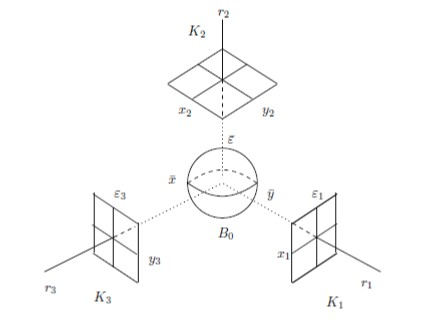
\includegraphics[height=5cm,width=7cm]{Images/charts-ball}
	\caption{Three charts mapping different sections of our blow up \citep{krupa2001}.}
	\label{fig:chartDiagram}
\end{figure}
In terms of the blown up fold point, a sphere denoted by $B$, charts are projections of regions of $B$ onto a two dimensional plane. 
We introduce three charts $ K_1,K_2,$ and $K_3 $. Chart $K_2$ is the two dimensional projection covering the upper half plane of $B$. However, as points on the equator of $B$ are approached on $K_1$, the point tends to infinity. These regions however, are of immense interest, since they are points of incoming and outgoing trajectories. As a consequence, charts $K_1$ and $K_3$ are introduced, covering the regions of interest on the equator of the fold point. 
%This is represented in Figure ++++++ (blow up figure)++
%The points that are relevant to the analysis of the dynamics are shown in Figure (+++insert figure 2.2 p,293+++++). (More description potentially)
The charts are defined by setting each of the variables of the extended system to $1$ in turn, giving $ \bar{y}=1, \ \bar{\epsilon}=1, \ \bar{x}=1 $. Substituting these into Equations (\ref{sys: blow up trans x}), (\ref{sys: blow up trans y}) and (\ref{sys: blow up trans z}) respectively gives, 
\begin{subequations} \label{ sys: K1K2K3}
	\begin{align}
	&x=r_1x_1, \ y=r_1^2, \ \epsilon=r_1^3\epsilon_1, \label{sys: K1}\\
	&x=r_2x_2, \ y=r_2^2y_2, \ \epsilon=r_2^3 \label{sys: K2}\\
	&x=r_3, \ y=r_3^2y_3, \ \epsilon=r_3^3\epsilon_3\label{sys:K3}
	\end{align}
\end{subequations}
where $ (x_i,r_i,\epsilon_i)\in\mathbf{R}^3 $ for $ i=1,2,3 $, and the equations correspond to the charts in numerical order \citep{krupa2001}. 
With this setup, we can consider the individual charts in turn, analyse the dynamics on the individual charts, and then join the gathered information into a global view on the dynamics in $U$.
We start with $K_2$,  because it holds the most information and the flow is the analysed more readily than in the other two charts. 
The remaining question is how the transition between the three charts and the connection to the global dynamics is made after finishing the individual analysis.
This is done via a coordinate change, derived by using Equations \ref{ sys: K1K2K3} and \ref{sys: blow up trans}, and the results are summarised in the following Lemma:
\begin{lemma} \label{coord. change}
Let $\kappa_{12}$ denote the change of coordinates from $K_1$ to $K_2$. Then $\kappa_{12}$ is given by \\
\begin{equation*}
x_2 = x_1 \epsilon_1^{-1/3},  y_2 = \epsilon_1^{-2/3}, r_2= r_1\epsilon_1^{1/3},
\end{equation*}
for $\epsilon_1 >0$,
and $\kappa_{12}^{-1}$ is given by
\begin{equation*}
x_1 = x_2y_2^{-1/2}, r_1 = r_2 y_2^{1/2}, \epsilon_1= y_2^{-3/2},
\end{equation*}
for $y_2>0$.
Let $\kappa_{23}$ denote the change of coordinates from $K_2$ to $K_3$. Then $\kappa_{23}$ is given by
\begin{equation*}
r_3 = r_2x_2, y_3= y_2x_2^{-2}, \epsilon_3 = x_2^{-3}, \label{eq:kappa23}
\end{equation*}
for $x_2>0,$
and $\kappa_{23}^{-1}$  is given by
\begin{equation*}
x_2 = \epsilon_3^{-1/3}, y_2 = y_3\epsilon_3^{-2/3}, r_2= r_3 \epsilon_3^{1/3},
\end{equation*}
for $\epsilon_3>0$.
\end{lemma}

Furthermore, transition maps $\Pi_i, i \in 1,2,3$  are defined in each section, describing how the trajectories coming in and out of each chart. These are combined in the final part of this section to give the proof of Theorem \ref{transition map theorem}, and to relate the results of the blow up method back to the original transition map $\pi$.
\newpage
\subsection{Dynamics in \texorpdfstring{$K_2$}{K2}} \label{sec: VDP K2}
\begin{figure}[h!]\centering
	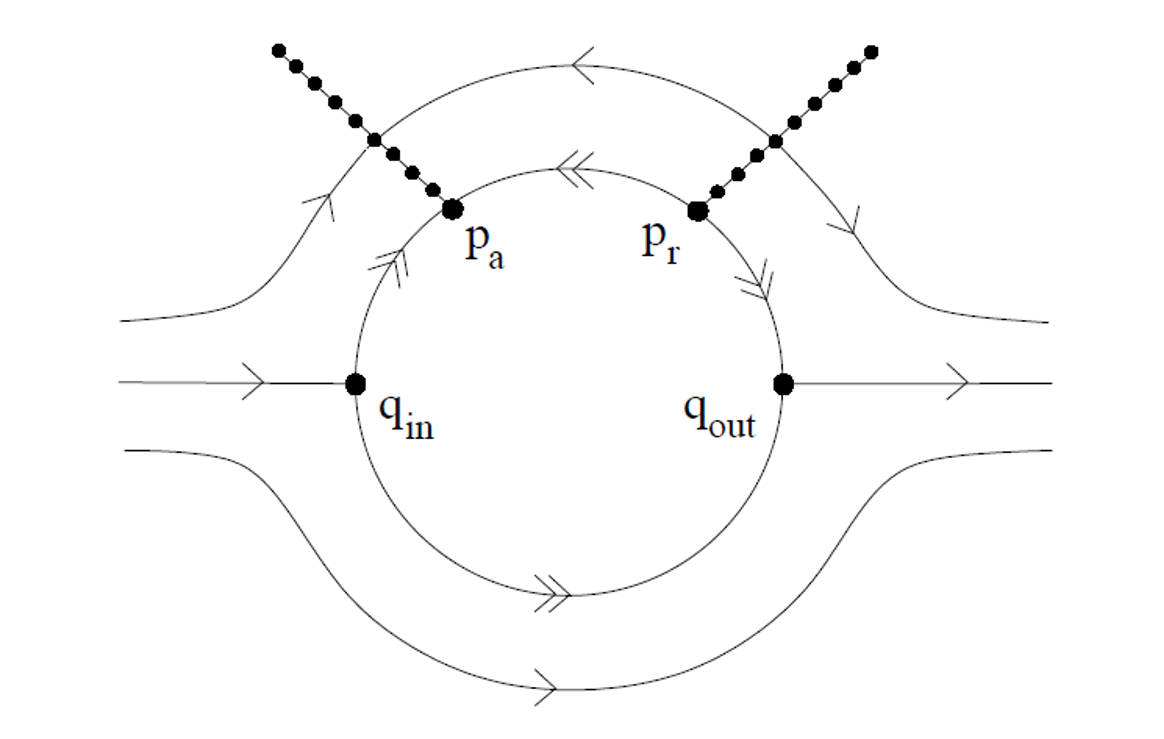
\includegraphics[height=4cm,width=6cm]{Images/Dynamics_in_Chart_2}
	\caption{Phase portrait for chart 2 \citep{krupa2001}.}
	\label{fig: chart 2 fig}
\end{figure}
To be able to consider chart $ K_2$, the transformation presented in Equation \ref{sys: K2} is applied to the extended system (\ref{extended FS}). Furthrmore,a time rescaling ($ t_2=r_2t $) is applied to desingularise the system. This results in:
\begin{equation}
	\begin{aligned}
		&\od{}{t}(r_2x_2)=r_2^2\od{x_2}{t}=-y_2+x_2^2-\dfrac{x_2^3r_2}{3},\\
		&r^3_2y'_2=r^3_2(-1+r_2x),\\
		&r'_2=0,
	\end{aligned}
\end{equation}
noting that $ \od{r}{t_2}=\od{t}{t_2}\od{r}{t}=\frac{1}{r_2}\od{r_2}{t} $ .  Now dividing through by $ r^2_2 $ and $ r^3_2 $ respectively for each equation and grouping $O(r_2)$ terms we get,
\begin{equation}
	\begin{aligned}
		&x'_2=x^2_2-y_2+O(r_2),\\
		&y'_2=-1+O(r_2),\\
		&r'_2=0.
	\end{aligned}
\end{equation}
Then, considering $r_2=0$ and neglecting the $O(r_2)$ terms results in,
\begin{equation} \label{Riccati}
	\begin{aligned}
		&x'_2=x^2_2-y_2,\\
		&y'_2=-1,\\
	\end{aligned}
\end{equation}
which are the well known Riccati equations- see \citet{Riccati}.
Some known results about the Riccati equations can be summarised as follows:


\begin{prop}[\citealp{krupa2001}]\label{Riccati Prop} 
The Riccatti equation (\ref{Riccati}) has the following properties:
\begin{enumerate}
\item Every orbit has a horizontal asymptote $y=y_r$, where $y_r$ depends on the orbit such that $x \to \infty$ as $y$ approaches $y_r$ from above.
\item There exists a unique orbit $\gamma_2$, which can be parameterized as $(x,s(x)), x \in \mathbf{R}$ and is asymptotic to the left branch of the parabola $x^2 - y = 0$, for $x \to - \infty$. The orbit $\gamma_2$ has a horizontal asymptote $y= - \Omega_0 <0$, such that $x \to \infty$ as $y$ approaches $-\Omega_0$ from above.
\item The function $s(x)$ has the asymptotic expansions
\begin{align*}
s(x) &= x^2 + \frac{1}{2x} + O\left( \frac{1}{x^4} \right), x \to -\infty,\\
s(x) &= -\Omega_0 + \frac{1}{x} + O\left( \frac{1}{x^3} \right), x \to \infty.
\end{align*}
\item All orbits to the right of $\gamma_2$  are backward asymptotic to the right branch of the parabola $x^2-y=0$.
\item All orbits to the left of $\gamma_2$ have a horizontal asymptote $y=y_l>y_r$, where $y_l$ depends on the orbit, such that $x \to -\infty$ as $y$ approaches $y_l$ from below.
\end{enumerate}
\end{prop}

The solutions to the Riccati equations, described in Proposition \ref{Riccati Prop}, are displayed in Figure. Note that the equation $x^2 - y=0$ is locally the critical manifold $S$ close to the fold point.%+++a bit wavy argument+++
The orbit $\gamma_2$, corresponds to the global trajectory $\gamma$, of the full system, which is the candidate trajectory connecting the slow flow on $S^a$ entering $U$ through $p_a$ to the fast fibres, exiting $U$ through $q_{out}$ - described by Figure \ref{fig: Ricatti Sol}. 
\begin{figure}[h!]\centering
	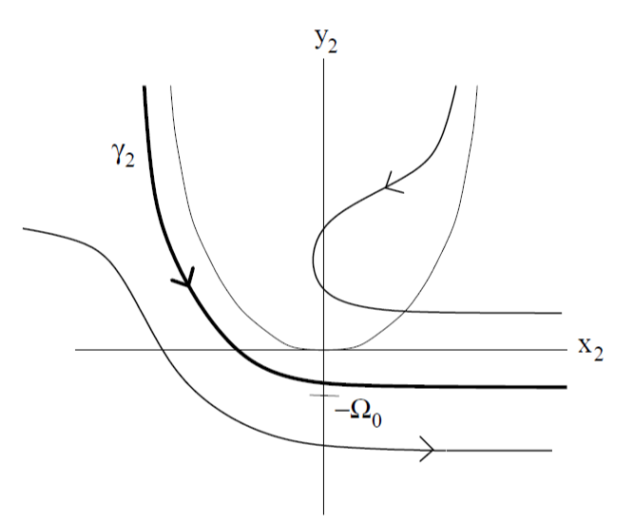
\includegraphics[height=6cm,width=6cm]{Images/Dynamics_in_K2}
	\caption{Ricatti solution for chart 2 \citep{krupa2001}.}
	\label{fig: Ricatti Sol}
\end{figure}
 
%(++++++refer back to figure  2.2 in krupa+++++++++)
This leads to the conclusion that if we can connect $\gamma_2$ to $p_a$  through $K_1$ and to $q_{out}$ through $K_3$, the global $\gamma$ can be constructed using Lemma \ref{coord. change}.
This motivates the analysis of $K_1$ and $K_3$.
In order to connect the dynamics on $K_2$ to that on the other charts, we need to define local inflow and outflow sections, similar to $\Delta^{in}$ and $\Delta^{out}$ in the full system.
Then we can follow trajectories that get mapped by $\Pi_2$, again analogous to $\pi$ in the full system, from a section $\Sigma^{in}_2$ to $\Sigma^{out}_2$.
The section are defined as follows. For $\delta>0$, we have:
\begin{align*}
\Sigma^{in}_2= \{ (x_2,y_2,r_2): y_2= \delta^{-2/3} \},\\
\Sigma^{out}_2 = \{ (x_2,y_2,r_2): x_2 = \delta^{-1/3} \}.
\end{align*}
Then the transition map $\Pi_2$ can be defined and the results are summarised as follows:
\begin{prop}[\citealp{krupa2001}]
The transition map $\Pi_2$ has the following properties:
\begin{enumerate}
\item
\begin{align*}
\Pi_2(q_0)= (\delta^{-1/3}, - \Omega_0 + \delta^{1/3} + O(\delta), 0)
\end{align*}
\item A neighbourhood of $q_0$ is mapped diffeomorphically onto a neighbourhood of $\Pi_2(q_0)$.
\end{enumerate}
\end{prop}
 
This is sufficient information to now consider the dynamics on $K_1$.

\subsection{Dynamics in \texorpdfstring{$K_1$}{K1}}\label{sec:dynamics-in-texorpdfstringk1k1} 
The coordinate transformation (\ref{sys: K1}) is applied to the extended system (\ref{extended FS}), 
\begin{align*}
\frac{d(r_1x_1)}{dt_1} \frac{dt_1}{dt} = -r_1^2 + r_1^2x_1^2 - \frac{1}{3}r_1^3x_1^3,\\
\frac{dr_1^2}{dt_1}\frac{dt_1}{dt}= 2r_1^2r_1' = r_1^3 \epsilon_1 (-1 +r_1 x_1),\\
\frac{d(r_1^3 \epsilon_1)}{dt_1}\frac{dt_1}{dt}= (3r_1^2\epsilon_1 + r_1^3 \epsilon_1') r_1 = 0.
\end{align*}
Dividing through by $\frac{dt_1}{dt}=r_1$ and replacing the expressions for $\epsilon_1'$ and $r_1'$ with their expressions in terms of the variables, results in the full system in terms of $K_1$. Note that the equation for $\epsilon'$ is found by rearranging the third equation above. 
\begin{align*}
x_1' &= -1 +x^2 + \frac{1}{2} x_1 \epsilon_1 + \left( - \frac{1}{2} \epsilon_1 x_1^2r_1 - \frac{1}{3} x_1^3 \right)\\
r_1' &= \frac{1}{2} r_1 \epsilon_1( -1 + r_1 x_1)\\
\epsilon_1' &= \frac{3}{2} \epsilon_1^2 ( 1- r_1x_1),
\end{align*}
and grouping terms in $r_1$ results in the standard form:
\begin{equation}
\begin{aligned} \label{K1systemfull}
x_1' &= -1 +x^2 + \frac{1}{2} x_1 \epsilon_1 +O(r_1)\\
r_1' &= \frac{1}{2} r_1 \epsilon_1( -1 + O(r_1))\\
\epsilon_1' &= \frac{3}{2} \epsilon_1^2 ( 1- O(r_1)).
\end{aligned}
\end{equation}

The system (\ref{K1systemfull}) has two invariant planes, that are somewhat equivalent to the notion of a nullcline. This tell us that the rate of change for our confidantes, $ r_1 $ and $ \epsilon_1 $ is constant for r$ _1=0 $ and $\epsilon_1=0$. If we substitute $r_1=0$ or $\epsilon_1=0$ into (\ref{K1systemfull}), the $r_1$ or $\epsilon_1$ equation respectively, are both zero, and there is only a two dimensional system left to consider. These two subspaces of (\ref{K1systemfull}) will be analysed below. Furthermore, the subspace where $r_1=0$ and $\epsilon_1=0$, is one dimensional, an invariant line, where the subspaces $r_1=0$ and $\epsilon_1=0$ cross.
The following analysis is displayed in Figure \ref{fig:k1chart}, illustrating the dynamics on $K_1$.
%\begin{figure}[h!]
%	\centering
%	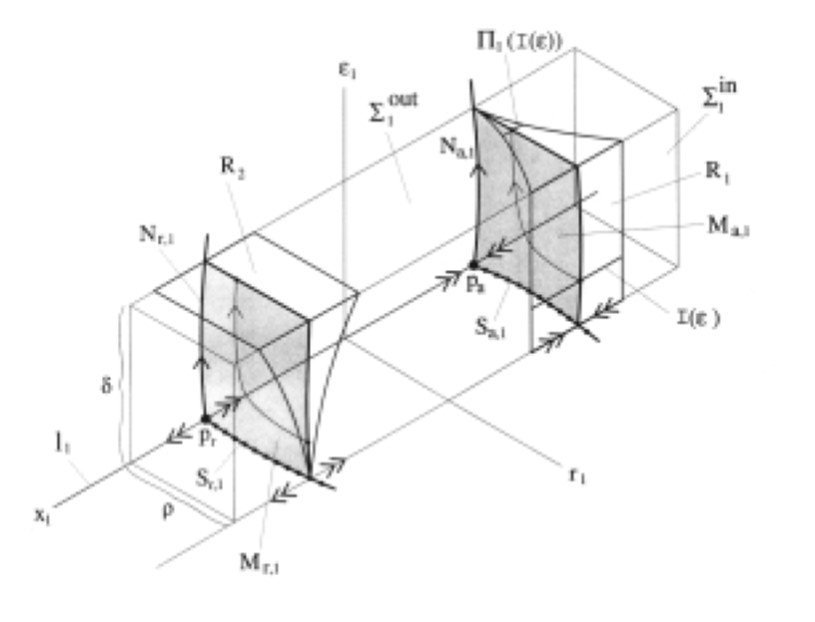
\includegraphics[width=7cm, height=7cm]{Images/K1Chart}
%	\caption{Dynamics in chart 1 \citep{krupa2001}
%	\label{fig:k1chart}
%\end{figure}
\begin{figure}[h!]
	\centering
	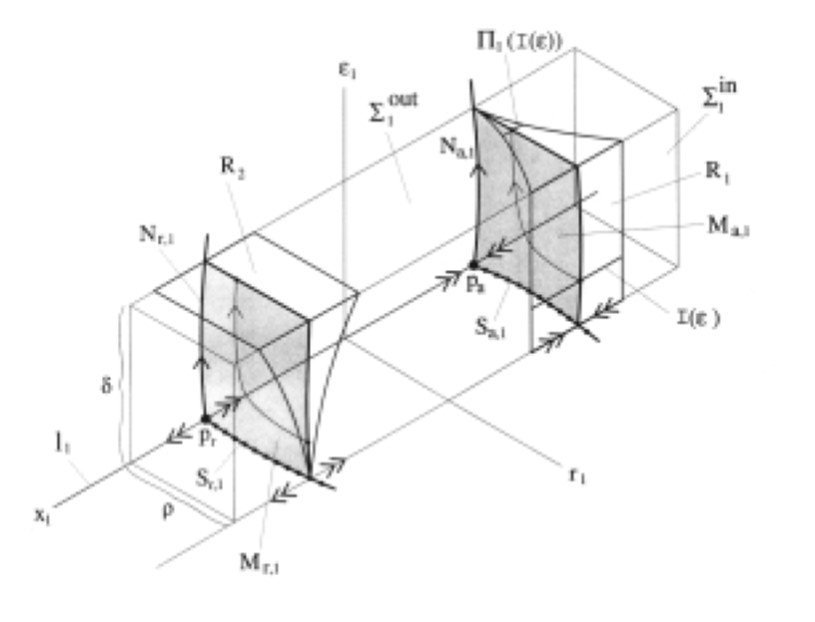
\includegraphics[height=7cm,width=7cm]{Images/K1Chart}
	\caption{Dynamics in chart 1 \citep{krupa2001}}
		\label{fig:k1chart}
\end{figure}\newpage


The invariant line, satisfying $r_1=0$ and $\epsilon_1=0$ is given by $l_1= -1 +x^2$. From this it is easily deduced that the two equilibrium points are where $l_1=0$, which is at $x=\pm1$. Therefore, the points $p_a$ and $p_r$ are defined as $p_a= (-1,0,0)$ and $p_r=(1,0,0)$. The flow on $l_1$ is attracted to $p^a$ and repelled by $p^r$, which is easily observed from the form $l_1$ takes or from a formal stability analysis of the one dimensional system. The eigenvalues of $l_1$ are found  by considering $l'_1 - \lambda = 2x - \lambda= 0 $ which gives that $\lambda = \pm 2$ at the respective equilibria. Then we expect the behaviour of the flow on the two invariant planes to be influenced by the two equilibria and the dynamics on $l_1$.
Consider the plane $\epsilon_1=0$. The system (Equation \ref{K1systemfull}) becomes
\begin{equation}
\begin{aligned} \label{epsilon0sys}
x_1' &= -1 +x_1^2 - \left( \frac{1}{3}r_1x_1^3 \right)\\
r_1' &= 0.
\end{aligned}
\end{equation}
This system has equilibria at $x= \pm1$, for $r_1=0$, as before, however, for each constant value of $r_1$, we get a different equilibrium of the system (\ref{epsilon0sys}). This forms a curve of equilibria, which can be recognised as $S^a_1$ connected to $p_a$ and $S^r_1$ connected to $p_r$, of the critical manifold, transformed into $K_1$ - this follows from the Implicit Function Theorem, see Figure \ref{fig: chart 2 fig}. The additional eigenvalue, corresponding to the $r_1$ equation, is $\lambda=0$. However, at each of the equilibria of this system, and specifically at $p_a$ and $p_r$ we have normal hyperbolicity, due to the coordinate transformation in $K_1$.% ++ go over this. +++
Next we consider the dynamics on the invariant plane $r_1=0$.
The system (Equation \ref{K1systemfull}) becomes: 
\begin{equation}
\begin{aligned}
x_1' &= -1 +x^2 + \frac{1}{2} x_1 \epsilon_1 \\
\epsilon_1' &= \frac{3}{2} \epsilon_1^2 .
\end{aligned}
\end{equation}
Again, $x= \pm 1$ are equilibria of the system, and an additional zero eigenvalue is gained due to the $\epsilon$ equation. It can be concluded that one dimensional centre manifolds exist, called $N_{a,1}$ and $N_{r,1}$, that are invariant, but not manifolds of equilibria like $S^a$ and $S^r$ in the $\epsilon=0$ plane. The dynamics on these manifolds are determined mainly by the value of $\epsilon$, since the change in the $\epsilon$ direction is much stronger than the change in the $x$ direction. Therefore, on $N_{a,1}$ and $N_{r,1}$ the flow moves in the $\epsilon$ direction with increasing epsilon.
In order to draw conclusions on the persistence of the dynamics in the full system, sections in the space are defined to monitor incoming and outgoing trajectories.
Firstly, let the region considered be such that
$D_1:= \{ (x_1,y_1,\epsilon_1): x_1 \in \mathbf{R}, 0, \leq r_1 \leq \rho, 0, \leq\epsilon_1 \leq \delta\}$.
Then the relevant sections for the candidate trajectory $\gamma$ are
\begin{align*}
\Sigma^{in}_1 := \{ (x_1,r_1, \epsilon_1) \in D_1 : r_1 = \rho \}, \\
\Sigma^{out}_1 := \{ (x_1,r_1, \epsilon_1) \in D_1 : \epsilon_1=\delta \}.
\end{align*}
Note that $\Sigma^{in}_1 = \Delta^{in}$ and $\Sigma^{out}_1=\Sigma^{in}_2$.
The aim is to find the connection between $p_a$ and $\gamma_2$ in $K_2$. In order to establish this connection, the trajectory $\gamma_2$ has to be mapped onto $K_1$ using Lemma \ref{coord. change}. Recall from Section \ref{sec: VDP K2} that the form of the candidate trajectory is of the form $(x_2, s(x_2))$.
Therefore, the trajectory $\gamma_1$ satisfies:
\begin{align*}
(x_1, 0, \epsilon_1) = \left(x_2 \left(x_2^2 + \frac{1}{2x_2} + O\left(\frac{1}{x_2^4} \right) \right)^{-1/2}, 0, \left(x_2^2 + \frac{1}{2x_2} + O\left(\frac{1}{x_2^4} \right)\right)^{-3/2} \right).
\end{align*}
Note that $s(x_2)$ as $x_2 \to - \infty$ is employed, since we consider the left continuation of $\gamma_2$.
Furthermore, as is intuitively clear from Figure \ref{fig: Ricatti Sol}, and can be shown by analysing the form of $\gamma_1$, the trajectory $\gamma_1$ converges to $p_a$ in backward time, which is exactly as expected.
This establishes the link between the slow flow on $S^a$ and the flow on $K_2$, if we consider the following proposition, which sums up the findings in $K_1$ and employs center manifold theory in order to establish persistence in the full system.
\begin{prop}[\citealp{krupa2001}]
For $\rho, \delta$ sufficiently small the following assertions hold for the system \ref{K1systemfull}:
\begin{enumerate}
\item There exists an attracting two-dimensional $C^k$- center manifold $M_{a,1}$ at $p_a$ which contains the line of equilibria $S_1^a$ and the center manifold $N_{a,1}$. In $D_1$ the manifold $M_{a,1}$ is given as a graph $x_1=h_a(r_1,\epsilon_1)$. The branch of $N_{a,1}$ in $r_1=0, \epsilon_1>0$ is unique.
\item There exists a repelling two-dimensional $C^k$- center manifold $M_{r,1}$ at $p_r$ which contains the line of equilibria $S_1^r$ and the center manifold $N_{r,1}$. In $D_1$ the manifold $M_{r,1}$ is given as a graph $x_1=h_r(r_1,\epsilon_1)$. The branch of $N_{r,1}$ in $r_1=0, \epsilon_1>0$ is not unique.
\item There exists a stable invariant foliation $F^s$ which base $M_{a,1}$ and one-dimensional fibres. For any $c>-2$ there exists a choice of positive $\rho$ and $\delta$ such that the contraction along $F^s$ during a time interval $[0,T]$ is stronger than $e^{cT}$.
\item There exists an unstable invariant foliation $F^u$ which base $M_{r,1}$ and one-dimensional fibres. For any $c>-2$ there exists a choice of positive $\rho$ and $\delta$ such that the expansion along $F^u$ during a time interval $[0,T]$ is stronger than $e^{cT}$.
\item The unique branch $N_{a,1}$ in $r_1=0, \epsilon_1>0$ is equal to $\gamma_1:= \kappa^{-1}_{12}(\gamma_2)$ wherever $\kappa^{-1}_{12}(\gamma_2)$ is defined, i.e. along the part of $\gamma_2$ corresponding to $y_2>0$.
\end{enumerate}
\end{prop}
 
In order to find the lower bound on the contraction rate along $F^s$, the transition time $T$  has to be found, i.e. the time the trajectory takes to travel from a point $p= (x_1, \rho, \epsilon_1)  \in \Sigma^{in}_1$ to a point in $\Pi_1(p)=( x_1, r_1, \delta) \in \Sigma^{out}_1$. This is done by integrating the $\epsilon$ equation of system (\ref{K1systemfull}), which is a separable ODE with respect to $t_1$.
This then results in 
\begin{align*}
T= \frac{2}{3} \left(\frac{1}{\epsilon_1} - \frac{1}{\delta} \right) \left( 1 + O(\rho) \right),
\end{align*}
where $r_1= \rho \in p$. 
Therefore, a transition map $\Pi_1: \Sigma^{in}_1 \to \Sigma^{out}_1$ can be defined for small enough parameter values of $\rho, \delta, \beta_1$. We are interested specifically in the transition around the center manifolds $M_{a,1}$ and $M_{r,1}$. The following subsections of $\Sigma^{in}_1 $ and $ \Sigma^{out}_1$ can be defined. Let $R_1= \{ (x_1, \rho, \epsilon_1) : |1+ x_1| \leq \beta_1 \}$, a rectangle in the intersection of the manifolds $M_{a,1}$ and  $\Sigma^{in}_1 $, and $R_2= \{ (x_1, r_1, \delta) : |1- x_1| \leq \beta_1 \}$, a rectangle in the intersection of the manifolds $M_{r,1}$ and  $\Sigma^{out}_1 $, with $\beta_1 >0$ sufficiently small. 
Furthermore, we can define line segments in these rectangles as $I_a(\overline{\epsilon}) \subset R_1$ and $I_r(\overline{r}) \subset R_2$, where $0 \leq \overline{\epsilon} \leq \delta$ and $0 \leq \overline{r} \leq \rho$.
Then for any $\overline{\epsilon}$, $\Pi_1$ maps the trajectory on a smaller region $\Pi_1 { I_a(\overline{\epsilon})} \in  \Sigma^{out}_1 $. This is called a contraction of the trajectories.
Considering Theorem \ref{transition map theorem}, which states the dependence of the contraction rate on $\epsilon$, the bounds on the contraction rate can be related to $\epsilon$, the parameter of the original system. Then using the $K_1$ rescaling of $\epsilon= \epsilon_1 r_1^3$, see Equation \ref{sys: K1},  the contraction rate for $\Pi_1 |I_r(\overline{r})$ is found by replacing $\epsilon_1$ by $\frac{\delta r^3_1}{\rho^3}$. 
Visual understanding of this analysis can be gained by considering Figure \ref{fig:k1chart}.
%++++ contraction in$ I_r$???+++++ 
The following proposition summarises the the findings for $\Pi_1$:
\begin{prop}[\citealp{krupa2001}]
For $\rho, \delta$ and $\beta_1$ sufficiently small, the transition map $\Pi_1: \Sigma^{in}_1 \to \Sigma^{out}_1$ defined by the flow of system \ref{K1systemfull} has the following properties:
\begin{enumerate}
\item $\Pi_1(R_1)$ is a wedge- like region in $\Sigma^{out}_1$. $\Pi_1^{-1}(R_2)$  is a wedge- like region in $\Sigma^{in}_1$.
\item More precisely, for fixed $c<2$, there exists a constant $K$ depending on the constants $c, \rho, \delta$ and $\beta_1$ such that:
\begin{enumerate}
\item for $\overline{\epsilon}\in (0, \delta] $ the map $\Pi_1 |I_a(\overline{\epsilon})$ is a contraction with contraction rate bounded by $Ke^{-\frac{2c}{3} \left(\frac{1}{\overline{\epsilon}} - \frac{1}{\delta} \right)}$.
\item for $\overline{r} \in (0, \rho] $ the map $\Pi_1 |I_r(\overline{r})$ is a contraction with coontraction rate bounded by $Ke^{-\frac{2c}{3} \left(\frac{\rho^3}{r_1^3 \delta} - \frac{1}{\delta} \right)}$.
\end{enumerate}
\end{enumerate}
\end{prop}

\subsection{Dynamics in \texorpdfstring{$K_3$}{K3}}\label{sec:dynamics-in-texorpdfstringk3k3}
The final chart to study the behaviour of is $K_3$. This chart covers the trajectory as it leaves the fold point at $q_{out}$. The other charts could not do this as $q_{out}$ is close to infinity in both $K_1$ and $K_3$ (cf. Figure \ref{fig:chartDiagram}). Similarly to $K_1$ and $K_2$, the system can be analysed using the blow-up transformation (\ref{sys:K3}).
\begin{subequations}
	\begin{align}
	\od{r_3}{t_3}&=r_3F(r_3,y_3,\epsilon_3) \\
	\od{y_3}{t_3}&=\epsilon_3(r_3-1)-2y_3F(r_3,y_3,\epsilon_3)\\
	\od{\epsilon_3}{t_3}&=-3\epsilon_3F(r_3,y_3,\epsilon_3)
	\end{align}
	\label{sys:K3blowup}
\end{subequations}
where $F(r_3,y_3,\epsilon_3)=\left(1-y_3-\frac{r_3}{3}\right)$. Note that as $\epsilon_3$ and $r_3$ appear as a factor in their respective derivatives, the planes $\epsilon_3=0$ and $r_3=0$ are invariant and, by extension, so is the $y_3$ axis.
The aim is to continue the special trajectory found in the other two charts and to find the transition map in and out of this chart. We will then be able to construct a phase portrait for the whole space by combining the dynamics in each chart. Linearising the system about $(0,0,0)=q_{out}$ gives 

\begin{align*}
\begin{pmatrix}\dot{r}_3\\\dot{y}_3\\\dot{\epsilon}_3\end{pmatrix}= \begin{pmatrix}
1 & 0 & 0 \\ 
0 & -2 & -1 \\ 
0 & 0 & -3
\end{pmatrix} \begin{pmatrix}
r_3 \\ 
y_3 \\ 
\epsilon_3
\end{pmatrix} 
\end{align*}
As the matrix is upper triangular, its eigenvalues are trivially  $\lbrace 1,-2,-3\rbrace$ with corresponding eigenvectors $\lbrace (1,0,0),(0,1,0),(0,1,1)\rbrace$. This presents an issue as there is additive resonance i.e. $\lambda_2-(\lambda_1+\lambda_3)=0$.  This means the Poincar\'e-Dulac theorem does not hold and the vector field is not linearisable, there is no smooth transformation between the nonlinear and linear flow. Despite this, progress can still be made as the form of the equations allow a near identity transformation and yields the lowest order approximation to the flow. %Note that $q_{out}$ is also  a hyperbolic equilibrium of the system.  +++Mention $\bar{M}_a$, the locally invariant perturbation of the center manifold $M_a$? Passes near the delicate equilibrium point $q_{out}$ so behaviour very much depends on how we pass this point. +++\\
The special orbit, $\gamma_2$, can be mapped into this chart using the change of coordinates $\kappa_{23}$ of Equation \ref{eq:kappa23}.
$$\gamma_3=\kappa_{23}(\gamma_2)$$
In fact, $\gamma_3$ lies in the plane $r_3=0$ and converges to $q_{out}$ as $\epsilon \to 0$. To find the flow in a neighbourhood of $q_{out}$ we use sections similar to those introduced in $K_2$.

\begin{align*} \Sigma_3^{in} =\lbrace(r_3,y_3,\epsilon_3) &: r_3\in[0,\rho], y_3 \in [-\beta_3,\beta_3], \epsilon_3=\delta\rbrace,\\
\Sigma_3^{out} =\lbrace(r_3,y_3,\epsilon_3) &: r_3=\rho, y_3 \in [-\beta_3,\beta_3], \epsilon_3\in[0,\delta]\rbrace
\end{align*}

We now wish to find the transition map $\Pi_3$ between these two charts. That is, given that the trajectory enters somewhere in $\Sigma_3^{in}$, how will it behave until it reaches $\Sigma_3^{out}$? To do this, the system \ref{sys:K3blowup} will be studied after some simplification. The system is in fact equivalent to the Riccati equation. Observe that $F(r_3,y_3,\epsilon_3)\big|_{q_{out}} = 1-y_3 + O(r_3)\big|_{q_{out}} \approx 1 $. Thus dividing (\ref{sys:K3blowup}) through by $F$ yields
\begin{subequations}
	\begin{align}
	\dot{r}_3&=r_3\\
	\dot{y}_3&=-2y_3 - \frac{\epsilon_3}{1-y_3}+r_3\epsilon_3 G(r_3,y_3,\epsilon_3)\\
	\dot{\epsilon}_3 &= -3\epsilon_3
	\end{align}
	\label{eq:K3ricc}
\end{subequations}

In the invariant plane $r_3=0$, the system becomes the Riccati equation (cf. (\ref{Riccati})) transformed into the chart $K_3$ and with a rescaling of time.
\begin{align*}
y'_3 &= -2y_3-\frac{\epsilon_3}{1-y_3}\\
\epsilon'_3 &= -3\epsilon_3
\end{align*}
This system has eigenvalues $\lbrace -2,-3\rbrace$ and the issue of additive resonance has been avoided so we are able to linearise the system using a near-identity transformation. This transformation allows the elimination of awkward higher order terms (in this case, $\frac{1}{1-y_3}$). Let
$$y_3=\psi(\tilde{y}_3,\epsilon_3)=\tilde{y}_3+O(\tilde{y}_3\epsilon_3).$$
Let $\tilde{\psi}$ denote the inverse transformation and both be $C^k$ functions. The system (\ref{eq:K3ricc}) can now be linearised and the following proposition gives the transition map.

\begin{prop}[\citealt{krupa2001}]
	The transition map $\Pi_3$ for the transformed $K_3$ system (\ref{sys:K3blowup}) is
	$$ \Pi_s(r_3,y_3,\delta) = \begin{pmatrix}
	\rho \\ 
	\Pi_{32}(r_3,y_3,\delta) \\ 
	\left(\frac{r_3}{\rho}\right)^3\delta
	\end{pmatrix} $$ 
	where $$\Pi_{32}(r_3,y_3,\delta)=\left(\bar{\psi}(y_3,\delta)-\delta\right)\left(\frac{r_3}{\rho}\right)^2 + O(r^3_3\ln r_3)$$
\end{prop}
\begin{proof}
	We will use the near-identity transformation to find the passage time $T$ and thus the values of $r_3,y_3,\epsilon_3$ at this time. For brevity, the subscripts will be omitted for the remainder of this proof. Under the near-identity transformation, system (\ref{eq:K3ricc}) becomes
	\begin{subequations}
		\begin{align}
		\dot{r} &= r,\label{sys:K3riccNIr}\\
		\dot{\tilde{y}}&=-2\tilde{y}+\epsilon+r\epsilon H(r,\tilde{y},\epsilon)\label{sys:K3riccNIy}\\
		\dot{\epsilon} &= -3\epsilon
		\label{sys:K3riccNIeps}
		\end{align}
	\end{subequations}
	Let the subscript $i$ denote the value of a variable at its entry into the chart, and likewise $o$ for out. Then $(r_i,y_i,\epsilon_i)\in \Sigma^{in}$, and $(r_o,y_o,\epsilon_o)\in \Sigma^{out}$. Thus 
	$$\begin{array}{c c c}
	r(0)=r_i & &r(T)=r_o=\rho\\
	y(0)=y_i & &y(T)=y_o\\
	\epsilon(0)=\epsilon_i=\delta& & \epsilon(T)=\epsilon_o
	\end{array}
	$$
	We wish to construct an equation for the out variables $(T,\tilde{y}_o,\epsilon_o)$ in terms of the in variables $ (r_i,\tilde{y}_i) $, that is the transition map. The $r$ and $\epsilon$ equations are easily solved:
	\begin{align}
	r&=r_ie^t &&\epsilon=\delta e^{-3t}
	\end{align}
	Then using $r(T)=\rho$, 
	$$r(T)=\rho=r_ie^-t \implies T=\ln\left(\frac{\rho}{r_i}\right).$$
	
	For the equation in $y$, a little more work is required. We introduce a new coordinate $z$ as follows, $\tilde{y}=e^{-2t}(\tilde{y}_i-\delta+z)+\delta  e^{-3t}$. Upon first sight, this seems unlikely to be of any use. However, it turns out that this transformation is ideal as it allows many terms to be removed. First rearrange for $z$ and differentiate with respect to $t$.
	\begin{align*}
	&z=e^{2t} (\tilde{y}-\delta e^{-3t})-\tilde{y}_i+\delta\\
	&\od{z}{t}= 2e^{2t}\tilde{y}+e^{2t}\dot{\tilde{y}}+\delta e^{-t}
	\end{align*}
	Substitute $\dot{\tilde{y}}$ from Equation (\ref{sys:K3riccNIy}) and cancel terms. 
	\begin{align*}
	&=e^{2t}(-\epsilon+r\epsilon H(r,\tilde{y},\epsilon))+\delta e^{-t}\\
	&=-\epsilon e^{2t}+e^{2t}r\epsilon  H(r,\tilde{y},\epsilon) + \delta e^{-t}\\
	&=e^{2t}r\epsilon  H(r,\tilde{y},\epsilon)
	\end{align*}
	This final equality follows from the explicit solutions in $r$ and $\epsilon$ above. These equations also show that $r\epsilon e^{2t} = r_i\delta e^{-2t}e^{2t}$. Finally,
	$$\dot{z} = r_iH^z(\,r_i,\tilde{y}_i,t)$$
	where $H^z$ is the same as $H$ but under the transformation from $z$, i.e. $H^z(\,r_i,\tilde{y}_i,t) = \delta H(r_ie^t,e^{-2t}(\tilde{y}_i-\delta+z)+\delta e^{-3t}, \delta e^{-3t})$. This has not affected the expression for the passage time $T$. +++Uniform boundedness of H implies?+++ Hence $z(T)=r_iO(T)=O(r_i\ln (\frac{\rho}{r_i}))$
	Using the initial definition of $z$, we recover an expression for $\tilde{y}(T)$.
	\begin{align*}
	\tilde{y}(T)&=e^{-2T}\left(\tilde{y}_i-\delta+O\left(r_i\ln\left(\frac{\rho}{r_i}\right)\right)\right)+\delta e^{-3T}\\
	&=(\tilde{y}_i-\delta)e^{-2\ln\frac{\rho}{r_i}}+e^{-2\ln\frac{\rho}{r_i}}O\left(r_i\ln\frac{\rho}{r_i}\right)+\delta \frac{r_i^3}{\rho^3}\\
	&=(\tilde{y}_i-\delta)\frac{r_i^2}{\rho^2}+O\left(\frac{r_i^3}{\rho^2}\ln\frac{\rho}{r_i}\right)
	\end{align*}
	We now have an expression for each of the out variables in terms of the initial conditions, albeit under a near-identity transformation. All that remains is to undo this transformation using the inverse map $\tilde{\psi}$.
	
	+++Undo transformation, explain $r$ and $\epsilon$ coordinates in prop. ThenDONE!+++
\end{proof}

\subsection{The Full Solution}
The analysis of the three charts, discussed in the Sections \ref{sec: VDP K2}-\ref{sec:dynamics-in-texorpdfstringk3k3}, provided a descripition of the dynamics on each of the charts, as well as theory to conclude the persistence of the dynamics in the full system.
The special trajectory $\gamma$ has been traced through all charts and in chart 1 it has been linked to the slow flow of $S^a$, while in chart 3 the connection to the fast flow has been made. Therefore, the fold point is indeed a jump point, or transition point, which connects the slow and fast dynamic.
These transition points can also be seen in the case of singular canards, which are treated in the following section.
The remaining issue is the transition of this special trajectory through the charts in order to have a solution of the full system. 
This is equivalent to finding the transition map $\pi$ from Theorem \ref{transition map theorem}.
Let $\Pi: \Sigma^{in}_1 \to \Sigma^{out}_3$ be the full transition map of the Blow-Up Transformation. Then it satisfies
\begin{align*}
\Pi := \Pi_3 \circ \kappa_{23} \circ \Pi_2 \circ \kappa_{12} \circ \Pi_1,
\end{align*}
where $\kappa$ is the change of coordinates defined in Lemma \ref{coord. change} and $\Pi_1, \Pi_2, \Pi_3$ are the transition maps in each chart.
Finally, reversing the blow up transformation gives the full transition map $\pi$ and therefore there exists a trajectory $\gamma$ in the blow down vector field connecting slow and fast flow.
With this analysis at hand we are now able to describe the full dynamics of the Van der Pol system when $\epsilon>0$ by analysing the singular limit $\epsilon \to 0$. 

The full result is visualised in Figure \ref{fig: vdp flow diagram}.
\begin{figure}[h!]\centering
		\begin{subfigure}[t]{0.45\textwidth}
			\centering
			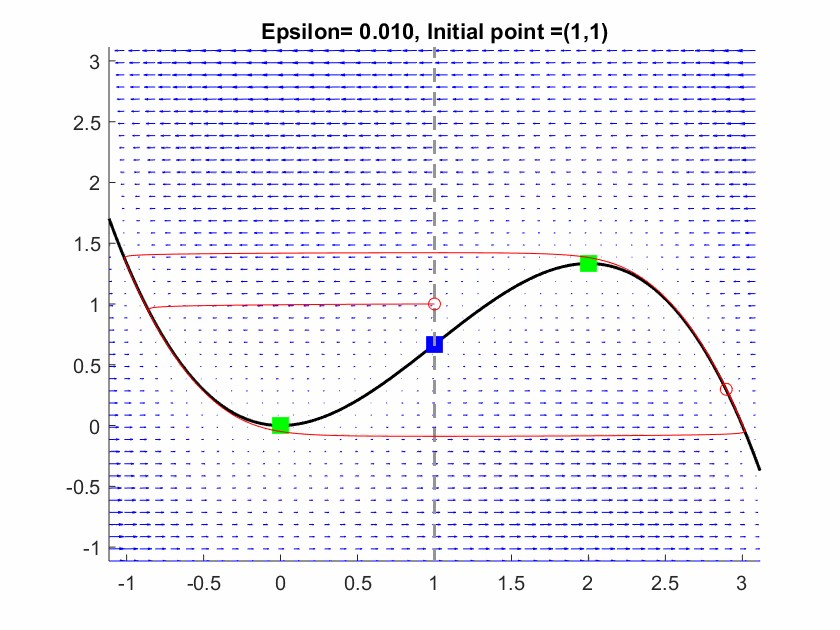
\includegraphics[width=.8\linewidth]{vdPe001-Moment-normal}
			\caption{The flow on the \vdp for a small $ \epsilon $.} \label{fig: vdp normal}
		\end{subfigure}
		\hfill
		\begin{subfigure}[t]{0.45\textwidth}
			\centering
			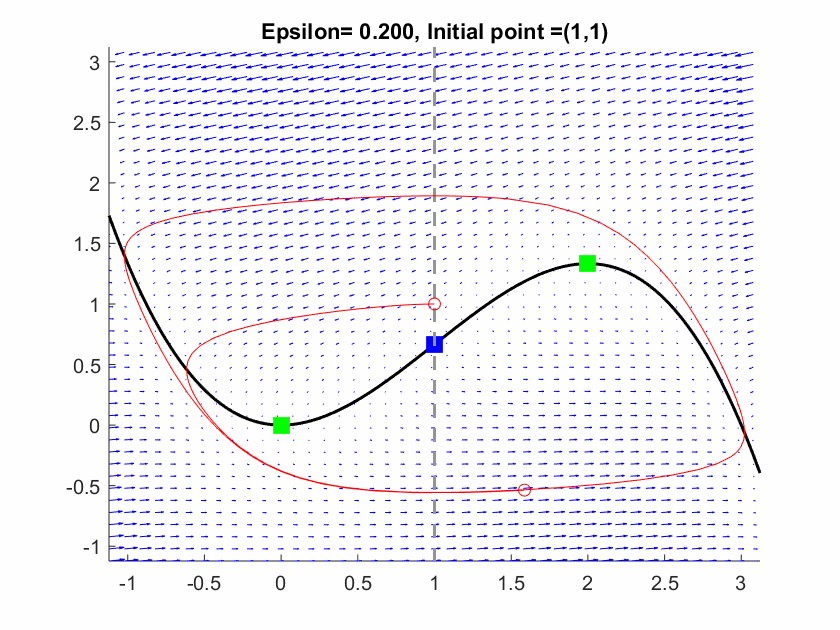
\includegraphics[width=.8\linewidth]{vdPe02-Moment-big-e}
			\caption{The flow on the \vdp for a larger $ \epsilon $.} \label{fig: vdp e.2}
		\end{subfigure}
		
%		\vspace{1cm}
%		\begin{subfigure}[t]{0.45\textwidth}
%			\centering
%			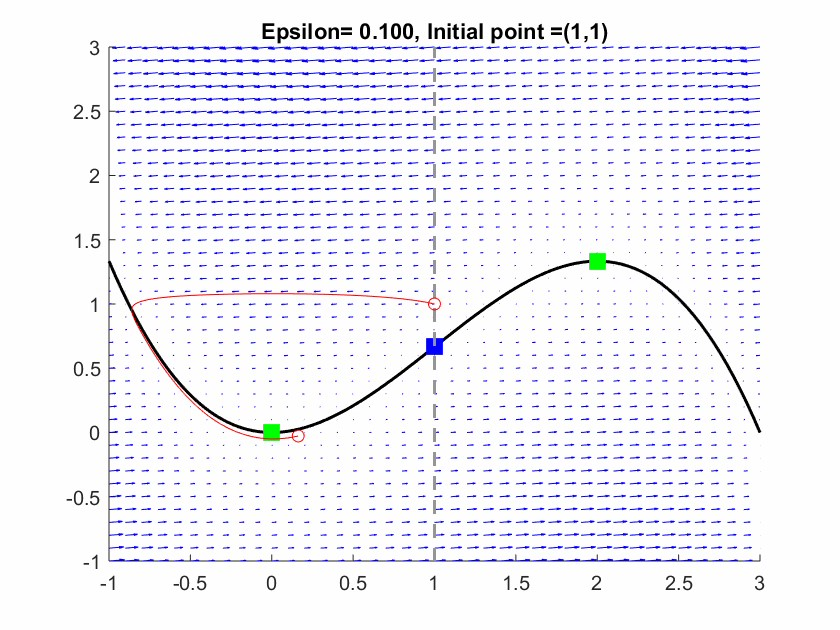
\includegraphics[width=.8\linewidth]{vdPhopf-Moment-3.jpg}
%			\caption{The flow as it intersects with the fold point.} \label{fig:timing3}
%		\end{subfigure}
%		\hfill
%		\begin{subfigure}[t]{0.45\textwidth}\centering
%			% just an empty subfigure to shift C below A
%			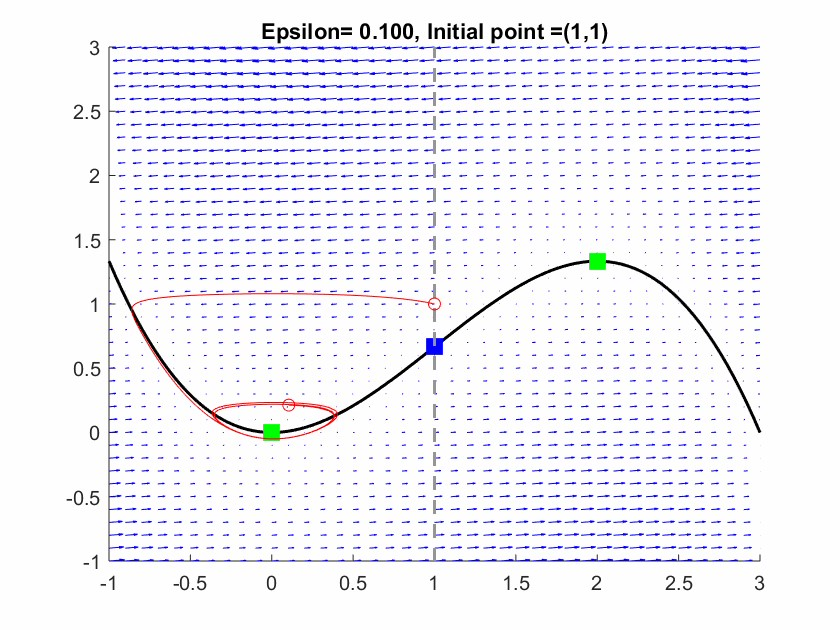
\includegraphics[width=.8\linewidth]{vdPhopf-Moment-4.jpg}
%			\caption{The Hopf bifurcation due to the canard point.}\label{fig:timing4}
%		\end{subfigure}
	\caption{Flow on the \vdp system.}
	\label{fig: vdp flow diagram e}
\end{figure}
++++ weave out +++++++++



























\section{Canard Points}
\begin{figure}[h!]
	\centering
	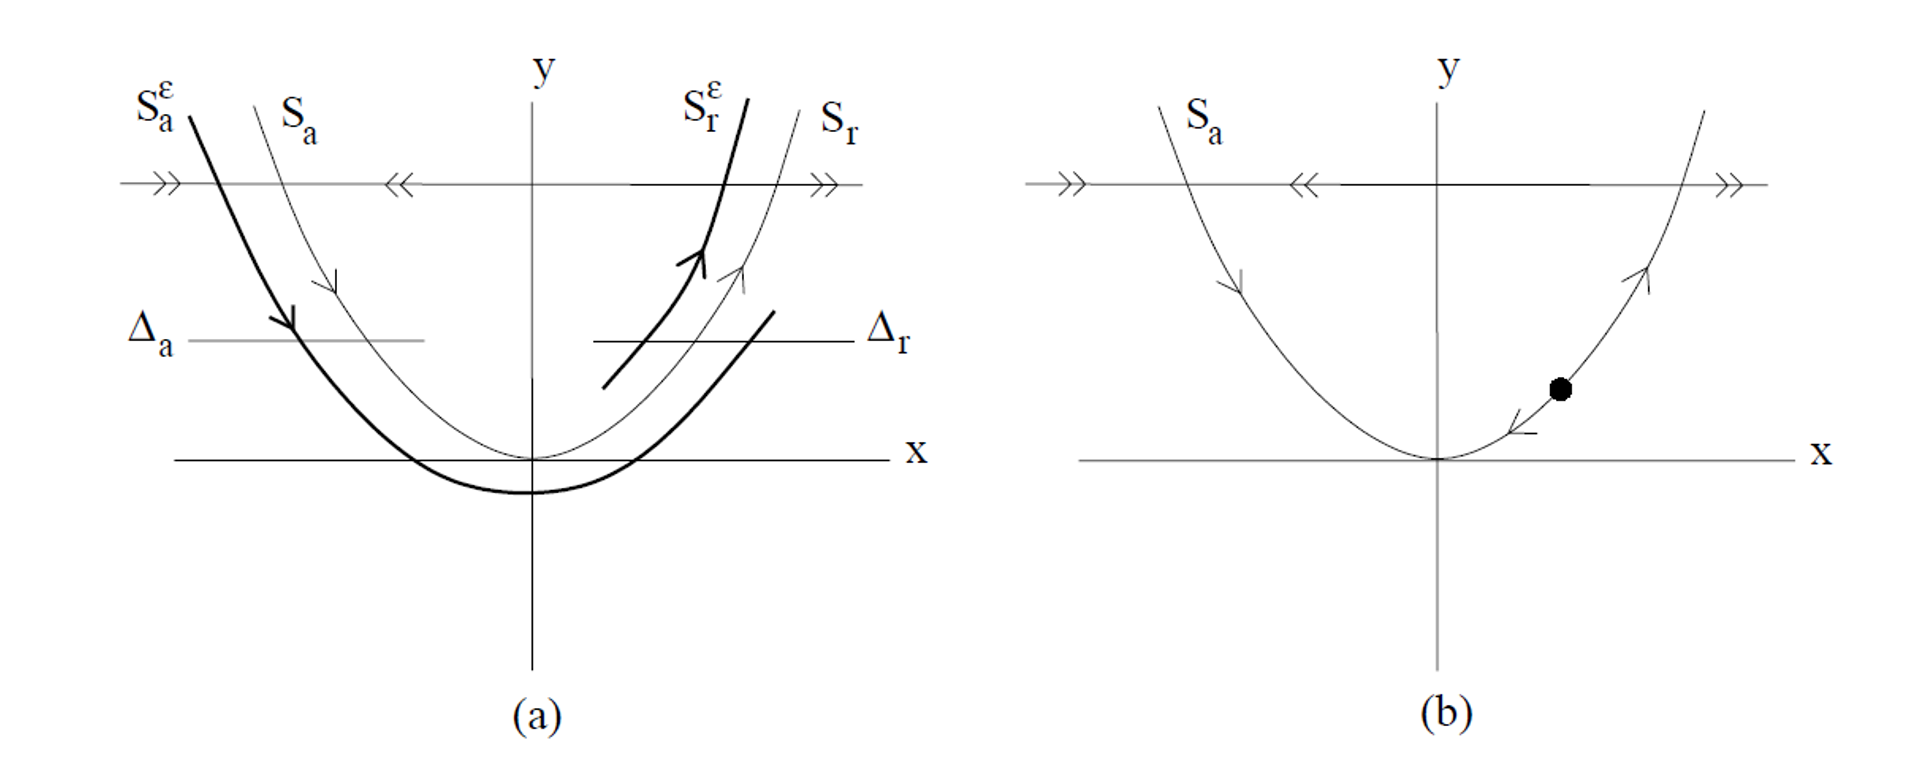
\includegraphics[height=5cm,width=8cm]{Canard_Point.png}
	\caption{The reduced flow where a) $\lambda=0$ and b) $\lambda>0$.}
	\label{fig: Canard Point}
\end{figure}\newpage



Considering the Van der Pol System as before:
\begin{equation}
\begin{aligned}
&x'=-y+x^2-\dfrac{x^3}{3},\\
&y'=\epsilon(x-1),\\
\end{aligned}
\tag{\ref{eq: Fast System}}
\end{equation}
we notice that the equilibrium of the system depends on the two nullclines $ x'=0$ and $y'=0$. These are in the shape of a cubic funcion and in the shape of a vertical line at $x=1$. 
The idea in this section is to replace the nullcline $x=1$ by $x = \lambda$. This can be seen as shifting the equilibrium of the system along the critical manifold $S$ by varying the parameter $\lambda$.
This gives rise to a generalised Van der Pol system:
\begin{equation}
\begin{aligned}
&x'=-y+x^2-\dfrac{x^3}{3},\\
&y'=\epsilon(x-\lambda).\\
\end{aligned}
\label{eq: canard system}
\end{equation}
In this section, the dynamics in system \ref{eq: canard system} is analysed. In order to do so, we need the definition of a canard.
\begin{definition}{\textbf{ Canard}}[\citealp{Kuehn}]
A trajectory of a fast-slow system is called a canard if it stays within $O(\epsilon)$ close to the repelling branch $S^r$ of the slow manifold $S$, for some time of $O(1)$ on the slow time scale $\tau = \epsilon t$.
\end{definition}
Furthermore, the following definition turns out to be useful as well:
\begin{definition}{\textbf{Maximal Canard}}[\citealp{Kuehn}] \label{maxcanard}
The trajectory passing through the intersection of $S^a$ and $S^r$ is called a maximal canard. 
\end{definition}
\begin{definition}{\textbf{Singular Canard}}
\end{definition}
The intuition of the canard problem close to a fold point is given in Figure \ref{fig: Canard Point}.
Equivalently to the analysis of the fold point in Section \ref{sec:the-van-der-pol-equation}, some nondegeneracy conditions are defined. These are, as before, applied at the fold point $(0,0)$. Note that in contrast to the nondegeneracy conditions in (\ref{NonDeg}), the transversality condition $g(0,0,0) \neq 0$ is not satisfied. Therefore higher order conditions on $g$ have to be employed, in particular these are nonzero derivatives of $g$ with respect to $x$ and $\lambda$. The fact that $g_x(0,0,0) \neq 0$ guarantees the existence of transversal intersection of the two nullclines, which is crucial in order to conclude persistence of the dynamics later on \citep{kuehn}. 
The nondegeneracy and transversality conditions for the canard case are  \citep{krupa2001},
\begin{equation}
f(0,0,0,0)=0, \ \pd{}{x}f(0,0,0,0)=0, \ g(0,0,0,0)=0, \label{eq: canard sing condition}
\end{equation}
\begin{equation}
\begin{aligned}
&\pd{^2}{x^2}f(0,0,0,0)\neq 0, \ \pd{}{y}f(0,0,0,0)\neq 0,\\
&\pd{}{x}g(0,0,0,0)\neq 0, \ \pd{}{\lambda}g(0,0,0,0)\neq 0. \label{eq: canard non-d condition}
\end{aligned}
\end{equation}
Now that these conditions have been defined we can consider, equivalent to the argument in Section \ref{sec: extended sys blowup}, the extended \vdp system,
\begin{equation}
\begin{aligned}
&x'=-y+x^2-\dfrac{x^3}{3},\\
&y'=\epsilon(x-\lambda),\\
&\epsilon'=0,\\
&\lambda'=0,\\
\end{aligned}
\label{eq: canard system}
\end{equation}
where the change in $\epsilon$ and $\lambda$ are constant. 
Now, for the remainder of the section, we apply the method of \citet{krupa2001} to the Van der Pol System. The canonical form for the Canard System is:
\begin{equation} \label{canardysy2var}
	\begin{aligned}
		x'&=-yh_1(x,y,\epsilon,\lambda)+x^2h_2(x,y,\epsilon,\lambda) + \epsilon h_3(x,y,\lambda,\epsilon)\\
                        &= -y + x^2 \left( 1- \frac{x}{3} \right),\\
		y'&=\epsilon(xh_4(x,y,\epsilon,\lambda)-\lambda h_5(x,y,\epsilon,\lambda) + y h_6(x,y,\lambda,\epsilon)) \\
                        &= \epsilon( x- \lambda).
	\end{aligned}
\end{equation}
It follows that $h_1 = 1$, $h_2 = 1-\frac{x}{3}$, $h_3=0$, $h_4 =1$, $h_5=1$ and $h_6=0$.
It is possible to find a $\lambda>0$, for which an equilibrium on the repelling branch $S_r$ exists for the reduced dynamics.
The following definition can be made in order to simplify the following computations:

\begin{align*}
a_1=\pd{}{x}h_3(0,0,0,0)=& 0 \ \ \
a_2=\pd{}{x}h_1(0,0,0,0)= 0\ \ \ 
a_3=\pd{}{x}h_2(0,0,0,0)=-\frac{1}{3}\\
a_4&=\pd{}{x}h_4(0,0,0,0)=0\ \ \
a_5=h_6(0,0,0,0)=0.
\end{align*}
Furthermore, we can define the quantity:
\begin{align*}
A=-a_2+3a_3-(2a_4+2a_5)=-1,
\end{align*}
which is important in the following analysis, in particular for $A \neq 0$ \citep{krupa2001}. 
Similar to the procedure in Section \ref{sec: VDP Blowup}, sections of the dynamical system can be defined, in order to monitor the in- and outgoing trajectories. In this case we are interested in two sections of the neighbourhood $U$, defined as in Section \ref{sec: VDP Blowup}, that monitor $S^a$ and $S^r$ close to the fold point.
Let $ \Delta_a = \{ (x,\rho^2), x \in  I_a \}$ and $\Delta_r= \{ (x,\rho^2), x \in  I_r \}$, where $I_a,I_r$ are intervals on the real line and $\rho$ is sufficiently small.
Futhermore, define $q_a$ to be the point on $\Delta_a$ that belongs to the attracting branch $S^a$, while $q_r$ is equivalently defined as the point on $\Delta_r$ that corresponds to $S^r$. Finally, we are in the position to define the transition map $\pi: \Delta^a \to \Delta^r$, compare to Section \ref{sec: VDP Blowup}.
Following this, \citet{krupa2001} discuss the existence of a critical value for $\lambda$ (denoted $\lambda_c$), where the two branches $S_r$ and $S_a$ must connect in a smooth fashion.  
The transition map $\pi$ has to map the point $q_a$ to $q_r$, if the branches are connected, and the trajectory passing through the fold point is called the maximal canard, see Definition \ref{maxcanard}
The following theorem describes the technical details involved, and some of the results are derived by the following analysis.
\begin{theorem}[\cite{krupa2001}]
	Assume that system (3.1) satisfies the defining non-degeneracy conditions (Equations \ref{eq: canard sing condition} and \ref{eq: canard non-d condition}) of a canard point. Assume that the solution $ x_0(t) $ of the reduced problem connects $ S_a $ to $ S_r $. Then there exists $ \epsilon_0 > 0 $ and a smooth function $\lambda_c(\sqrt{\epsilon})$ defined on $ [0, \epsilon_0] $ such that for $\epsilon \in (0, \epsilon_0)$ the following assertions hold:
	\begin{itemize}
		\item $ \pi(q_{a,\epsilon})=q_{r,\epsilon} $ iff $ \lambda=\lambda_c(\sqrt{\epsilon}) $.\\
		\item The function $ \lambda_c $ has the expansion
		 \begin{equation*}
			\lambda_c(\sqrt{\epsilon})=-\epsilon(\frac{a_1+a_5}{2}+\frac{A}{8})+O(\epsilon^\frac{3}{2}).
			\end{equation*}
			\item The transition map $\pi$ is defined only for $\lambda$ in an interval around $ \lambda_c(\sqrt{\epsilon}) $ of width $ O(\exp(-\frac{c}{\epsilon})) $ fo some $ c>0 $.
			$$ \pd{}{\lambda}(\pi(q_{a,\epsilon})-q_{r,\epsilon})|_{\lambda=\lambda_c(\sqrt{\epsilon})}>0  $$
		
	\end{itemize}
\label{Theorem 3.1}
\end{theorem}
%Consider Canard cycles and center manifolds / Freddy Dumortier, Robert Roussarie. for more details on canards in \vdp. ++++++Kieran, what do you mean here+++++
%



\subsection{Canard Blow-up}
Now similarly to Section \ref{sec: VDP Blowup}, we consider a transformations of the coordinate system in order to analyse the dynamics in the neighbourhood of the non-hyperbolic equilibrium induced by the canard point. %(++++++ is the eq. induced by lambda??++++).
 The transformations are taken from \citep{krupa2001} and are,
\begin{equation}
x=\bar{r}\bar{x}, \ y=\bar{r}^2y, \ \epsilon=\bar{r}^2\bar{\epsilon}, \ \lambda=\bar{r}\bar{\lambda}.
\end{equation}
Now that we have established these transformation, the charts $K_1$ and $K_2$ can be introduced,  but it is not necessary to consider the third chart, $K_3$. Since the attracting slow manifold connects to the repelling slow manifold, the flow will `bend back' from $K_2$ into $K_1$ instead of leaving the neighbourhood $U$ in the direction of the fast flow, which was described by $K_3$ in Section \ref{sec: VDP Blowup}. 
This pheonomenon can be observed in Figure \ref{fig: flow in canard}, where the trajectory stays close to $S^r$ after passing the fold point.
\begin{figure}[h!]
	\centering
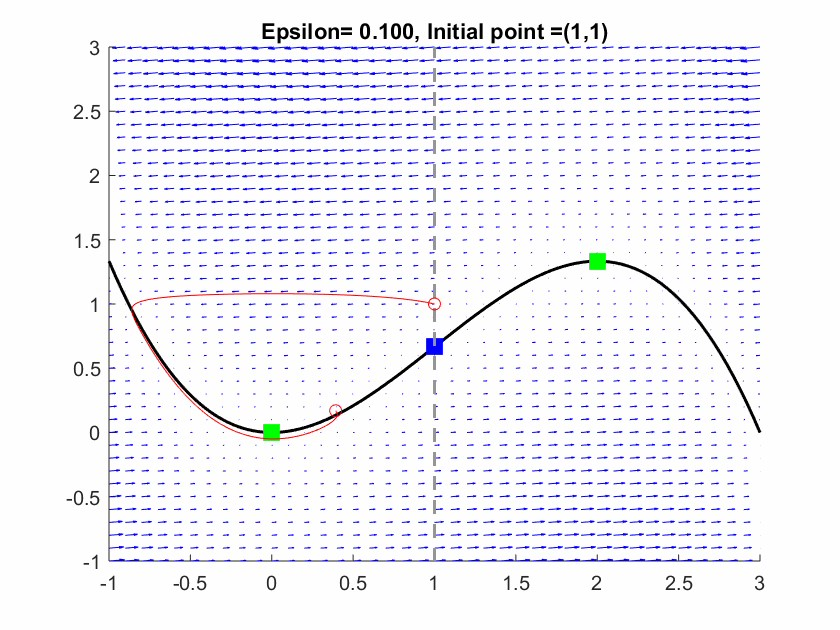
\includegraphics[width=8cm, height=6cm]{Images/vdPhopf-Moment-bendback}
	\caption{The \vdp system for the canard case.}
	\label{fig: flow in canard}
\end{figure}\newpage
Again, equivalently to the procedure in Section \ref{sec: VDP Blowup}, we can define the coordinate transformation for the charts. Note, that in contrast to the generic Blow-Up in Section \ref{sec: VDP Blowup}, the coordinate system is now in $\mathbf{R}^4$, and not in $\mathbf{R}^3$. In chart $K_1$, $y_1=1$, while in $K_2$, $\epsilon_1=1$ and then:
\begin{subequations}
	\begin{align}
	&x=r_1x_1, \ y=r_1^2, \ \epsilon=r_1^2\epsilon_1, \ \lambda=r_1\lambda_1 \label{eq: coordiante K1}\\ 
	&x=r_2x_2, \ y=r_2^2y_2, \ \epsilon=r^2_2, \ \lambda=r_2\lambda_2 \label{eq: coordinate K2}.
	\end{align}
\end{subequations}
Furthermore, we can define the coordinate change between the two charts as follows:
\begin{lemma}
Let $\kappa_{12}$ denote the change of coordinates from $K_1$ to $K_2$. Then $\kappa_{12}$ is given by
\begin{align*}
x_2 = x_1 \epsilon_1^{-1/2}, \ \ \ y_2 = \epsilon_1^{-1}, \ \ \ r_2 = r_1 \epsilon_1^{1/2}, \ \ \ \lambda_2 = \epsilon_1^{-1/2} \lambda_1,
\end{align*}
for $\epsilon_1 >0$.
Similarly $\kappa_{21}=\kappa_{12}^{-1}$ is given by
\begin{align*}
x_1 = x_2 y_2 ^{-1/2}, \ \ \ r_1 = r_2 y_2 ^{1/2}, \ \ \ \epsilon_1 = y_2^{-1}, \ \ \ \lambda_1 = \lambda_2 y_2^{-1/2},
\end{align*}
for $y_2 >0$.
\end{lemma}

We are now in the position to begin with the analysis in the charts, and will first consider chart $K_2$, since, as in Section \ref{sec: VDP Blowup}, $K_2$ holds the most information. 

\subsubsection{Dynamics in \texorpdfstring{$K_2$}{K2}}
%<<<<<<< HEAD
We start by noting that we are considering our invariant plane at $r_2=0$ which will significantly simplify our system for $K_2$. Further we should note that we are taking a transformation in time, $\od{r}{t_2}=\od{t}{t_2}\od{r}{t}=\frac{1}{r_2}\od{r_2}{t}$, as well as in our coordinates. Then if we substitute our time transformation and Equation  \ref{eq: coordinate K2} into our system of Equations \ref{eq: canard system} we find, 
\begin{subequations}
	\begin{align}
	r_2^2x_2' - r_2x_2r_2'&=-r_2^2y_2h_1+r^2_2x^2_2h_2,\notag\\
	\implies x'_2&=-y_2+x_2^2-r_2G_2(x_2,y_2), \label{eq k2 x trans}\\
	%     \end{aligned}
	% \end{equation*}
	% \begin{equation}
	%     \begin{aligned}
	r^3_2y_2'-3r_2^2y_2r_2'&=r^2_2(r_2x_2h_4-r_2\lambda_2h_5),\notag\\
	\implies y_2'&=x_2-\lambda_2+r_2G_2(x_2,y_2), \label{eq: K2 y trans}
	\end{align}
	\label{eq: reduced canard k2}
\end{subequations}
\noindent where we note that $h_j=h_j(x,y,\epsilon,\lambda)$ for $j=1,2,3,4,5$.  Notice that we have included an additional term in Equation \ref{eq: reduced canard k2} - we define $G_2(x_2,y_2)$ in the following way, $G(x_2,y_2)=(G_1(x_1,y_1),G_2(x_2,y_2))^T=(-\frac{x^3_2}{3},0)^T$. The reason we also define this vector is to aide in the Melnikov computations which we will see later. Then combing this yields our complete system
\begin{subequations}
	\begin{align}
	x'_2&=-y_2+x_2^2-r_2G_1(x_2,y_2) =-y_2+x_2^2-r_2\left(-\frac{x^3_2}{3} \right) ,\tag{\ref{eq k2 x trans}}\\
	y_2'&=x_2-\lambda_2+r_2G_2(x_2,y_2)= x_2-\lambda_2, %\label{eq: K2 y trans}
	\tag{\ref{eq: K2 y trans}}
	\end{align}
\end{subequations}
recalling that $r_2'=\lambda_2'=0$. Moreover, \citet{krupa2001} discusses that for this chart we have an interesting result. They note that at $r_2=\lambda_2=0$ our system is integrable which allows us to define a constant of motion $H(x_2,y_2)=\frac{1}{2}\exp{(-2y_2)}\left(y_2-x^2_2+\frac{1}{2}\right)$. For clarity we will first proceed with deriving this equation of motion. Firstly, multiply each equations by, $e^{2y_2}e^{-2y _2}=1$, and define sections of each equation as partial derivatives of $H$ \st, 
\begin{align}
x_2' &=e^{2y_2}e^{-2y_2}( -y_2 +x_2^2 ) =e^{2y_2}\pd{H}{y_2}(x_2,y_2) \\
y_2' &= - e^{2y_2}e^{-2y_2}(-  x_2)=-e^{2y_2}\pd{H}{x_2}(x_2,y_2).
\end{align}
Then we integrate $ \pd{H}{x_2}(x_2,y_2) = -e^{-2y_2} x_2  $ to give,
\begin{align*}
%&\Rightarrow H(x_2,y_2) = \int -e^{-2y_2} x_2 dx\\
 H(x_2,y_2) = - \frac{1}{2} x^2 e^{-2y_2} + C(y),
\end{align*}
where $C(y)$ is the constant of integration, which depends on $y$.
Then, by taking the derivative with respect to $y$ and setting it equal to the expression $\pd{H}{y_2}(x_2,y_2)=e^{-2y_2}( -y_2 +x_2^2 )$, we can find the value for $C(y)$ as follows: 
\begin{align*}
\pd{H}{y_2}(x_2,y_2)&= x^2 e^{-2y_2} + C'(y)\\
%&= e^{-2y_2}( -y_2 +x_2^2 )\\
\Rightarrow C'(y) &= - y_2 e^{-2y_2}
\end{align*}
Finally we integrate $C'(y)$ in order to find an explicit expression for $H$,
\begin{align*}
C(y) = \int - y_2 e^{-2y_2} dy = \frac{1}{2} y_2 e^{-2y_2} + \frac{1}{2} e^{-2y_2} + const,
\end{align*}
using integration by parts.
Then, the final expression is:
\begin{align}
H(x_2,y_2)&=- \frac{1}{2} x^2 e^{-2y_2} + \frac{1}{2} y_2 e^{-2y_2} + \frac{1}{2} e^{-2y_2} + c\\
&= \frac{1}{2}e^{-2y_2}\left(y_2-x^2_2+\frac{1}{2}\right) +c. \label{eq: const of motion}
\end{align}
Note that without loss of generality we can choose $c=0$ because we are interested in the level curves of $H$ and $H=h$. Now that we have shown how the constant of motion is constructed we will consider our reduced system, that we have an equilibrium at the origin, implying that $H(x_2,y_2)=h$. Considering the reduced system (Equation \ref{eq: reduced canard k2}) we have from $ H(x_2,y_2)=0 $ that,
\begin{subequations}
	\begin{align}
	x_2'&=\frac{1}{2}\ \	\implies x_2=\frac{t_2}{2}+A, \label{canard: trajectory x}\\
	y_2'&=\frac{t_2}{2}\ \implies y_2=\frac{t_2^2}{4}-\frac{1}{2}, \label{canard: trajectory y}
	\end{align}
\end{subequations} 
where we have directly integrated Equation \ref{canard: trajectory x} with respect to our time ($ t_2 $). However, we note that we are able to choose $ A=0 $, as we are considering an autonomous (time-invariant) system. Then for Equation \ref{canard: trajectory y} we are able to rearrange the constant of motion at zero to give, $ y_2=x_2^2-\frac{1}{2} $. Clearly from this analysis we are then able to define our trajectories in terms of $ \gamma_{c,2} $, 
\begin{equation}
\gamma_{c,2}(t_2)=(x_{c,2}(t_2),y_{c,2}(t_2))=\left(\frac{t_2}{2},\frac{t^2_2}{4}-\frac{1}{2}\right).   \label{eq: gamma c2}
\end{equation}
Now that we have established that we must have a flow on our second chart, then there must also exist transition maps. Therefore this now enables us to consider the first chart in the following section.


\subsubsection{Dynamics in \texorpdfstring{$K_1$}{K1}}\label{sec:dynamics-in-texorpdfstringk1k1}
For $K_1$ we follow a similar approach to the above. We will use the transformations, 
\begin{equation}
x=r_1x_1, \ y=r_1^2, \ \epsilon=r_1^2\epsilon_1, \ \lambda=r_1\lambda_1 \tag{\ref{eq: coordiante K1}},
\end{equation}
to find the relevant pathways of our flows. Now if we first consider the $r_1$ component, 
\begin{align}
2r_1^2r_1'=r_1^2\epsilon(r_1x_1-r_1\lambda_1), \label{canard: r1}
\end{align}
where we define $F=F(x,y,\epsilon,\lambda)=x_1-\lambda_1+O(r_1(r_1+\lambda_1)$. Next we consider $x=r_1x_1$,
\begin{align*}
r_1r_1'x_1+r_1^2x_1'&=-r_1^2+r_1^2x_1^2,\\
x_1'&=-1+x_1^2-\frac{x_1r_1'}{r_1},
\end{align*}
where we can use Equation \ref{canard: r1} to simplify this further,
\begin{align}
x_1'=-1+x_1^2-\frac{x_1}{r_1}\left(\frac{r_1\epsilon_1F}{2}\right). \label{eq: canard x1}
\end{align}
We now consider $\epsilon=\epsilon_1r_1^2$ and noting $\epsilon'=0$. Then we have, $r_1^3\epsilon'=-2r_1^2\epsilon_1r_1'$, where we can use Equation \ref{canard: r1} to simplify to,
\begin{align}
\epsilon'=-\epsilon_1^2F. \label{canard: epsilon k1}
\end{align}
Our last transformation is for our new coordinate $\lambda=r_1\lambda$, noting that $\lambda'=0$. Similarly to the above we find $r_1^2\lambda_1'+r_1\lambda_1r_1'=0$ then, 
\begin{equation}
\lambda'_1=-\frac{\lambda_1\epsilon_1F}{2}, 
\end{equation}
which is a trivial rearrangement as seen in Equation \ref{canard: epsilon k1}. Now if we combine the above we find that our transformed system is of the following form,
\begin{subequations}
	\begin{align}
	r_1'&=\frac{\epsilon}{2}(r_1x_1-r_1\lambda_1), \\
	% \label{canard: r1}
	x_1'&=-1+x_1^2-\frac{x_1\epsilon_1F}{2},\\
	\epsilon'&=-\epsilon_1^2F,\\
	\lambda'_1&=-\frac{\lambda_1\epsilon_1F}{2}.
	\end{align}
	\label{canard: system of equations}
\end{subequations}
From this system we are now able to make some deductions. We first can observe that the hyperplanes are along the $r_1=\epsilon_1=\lambda_1=0$ with an invariant line at $l_1=\{(x_1,0,0,0): x_1\in\mathbb{R}\}$ \citep{krupa2001}. As \citet{krupa2001} discusses the equilibria present at the end of both of our branches - Figure \ref{fig: Canard Point} - which are found at $p_a=(-1,0,0,0) \ \text{and} \ p_r=(1,0,0,0)$ \citep{krupa2001}. Now we can go one step further, we can consider Equation \ref{canard: system of equations} and find the eigenvalues of the system for the invariant planes. We find that, 
\begin{equation}
J-\sigma I= \begin{bmatrix}
2x-\sigma & 0 & 0 & 0  \\
0 & -\sigma & 0 & 0&\\
0 & 0 & -\sigma & 0 \\
0 & 0 & 0 & -\sigma
\end{bmatrix},
\end{equation}
which clearly has three zero eigenvalues and one non-zero eigenvalue $\sigma=\pm 2$. Which further empahsises that our equilibrium point is non-hyperbolic. As a result we intuitively expect that something interesting occurs at this point. In the section following we will be considering what effect these mappings and eigenvalues will have on our system.


\subsection{Effect of the Canard Point}\label{sec:effect-of-the-canard-point}
Now that we have shown that there must exist a flow around our fold point we should now consider the global effect of the canard point. We can see by considering the  system of Equations \ref{canard: system of equations} that our equilibriums are at $ (x,y)=(\lambda,\lambda^2[\frac{1-\lambda}{3}]) $ and find the eigenvalues from the matrix, 
\begin{equation}
A-\sigma I=\begin{bmatrix}
2x-x^2-\sigma&-1&0&0\\
\epsilon&-\sigma&x-\lambda&-\epsilon\\
0&0&-\sigma&0\\
0&0&0&-\sigma
\end{bmatrix}=\sigma^2(\sigma^2+\sigma(x^2-2x)+\epsilon).
\end{equation}
%\begin{equation}
%A-\sigma I=\begin{bmatrix}
%2\lambda-\lambda^2-\sigma&-1&0&0\\
%\epsilon&-\sigma&0&-\epsilon\\
%0&0&-\sigma&0\\
%0&0&0&-\sigma
%\end{bmatrix}.
%\end{equation}
%\textbf{Then our eigenvalues are, $ \sigma=(2-x)x \ \text{and} \ \sigma=0 $, noting that we have an upper triangular matrix. Then we can note that we have a complex eignevalue which causes a Hopf bifurcation, as shown below:}%wrong maths
From this we are about to find the eigenvalues of the system, $ \sigma=0 $ and $ \sigma=\frac{2x-x^2\pm\sqrt{(x^2-2x)^2-4\epsilon}}{2} $. Then we consider the values at our equilibrium, $ x=\lambda $, to find that we have a Hopf Bifurcation when $ 4\epsilon>(x^2-2x)^2 $ or when $ \lambda=2 \ \text{or} \ 0 $. This then leads to the following trajectories within the flow - Figure \ref{fig: 4 canard }.

\begin{figure}[h!]
	\centering
	\begin{subfigure}[t]{0.45\textwidth}
		\centering
		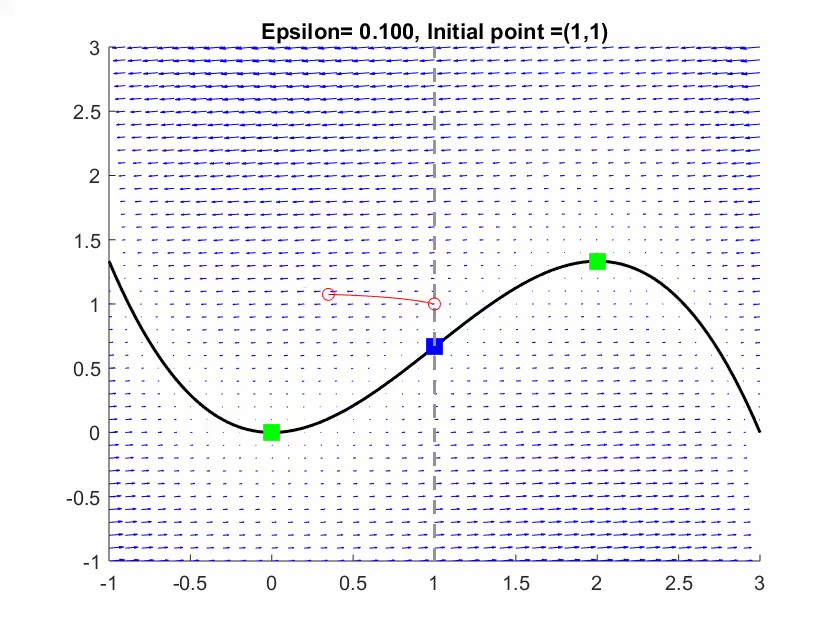
\includegraphics[width=.8\linewidth]{vdPhopf-Moment-1.jpg}
		\caption{The initial flow within the system.} \label{fig:timing1}
	\end{subfigure}
	\hfill
	\begin{subfigure}[t]{0.45\textwidth}
		\centering
		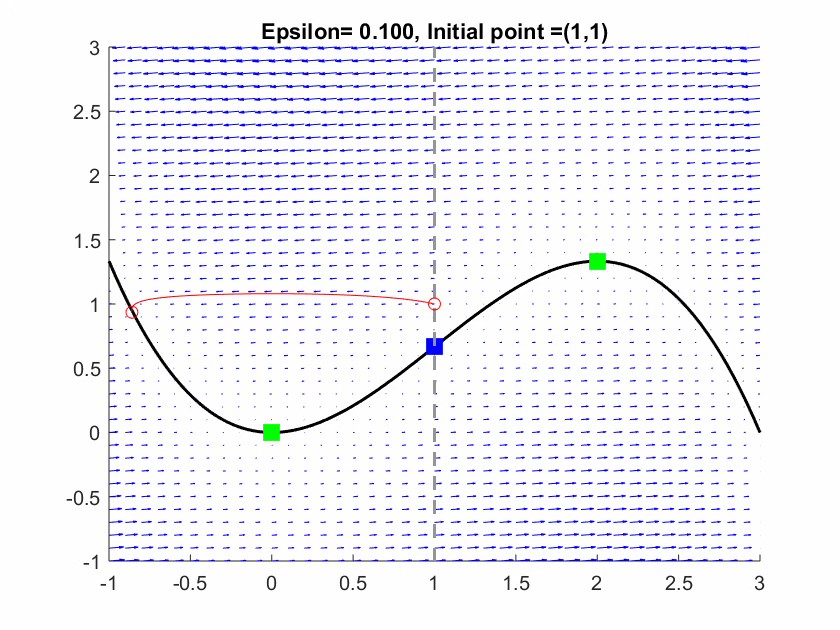
\includegraphics[width=.8\linewidth]{vdPhopf-Moment-2.jpg}
		\caption{The flow as it hits the slow manifold.} \label{fig:timing2}
	\end{subfigure}
	
	\vspace{1cm}
	\begin{subfigure}[t]{0.45\textwidth}
		\centering
		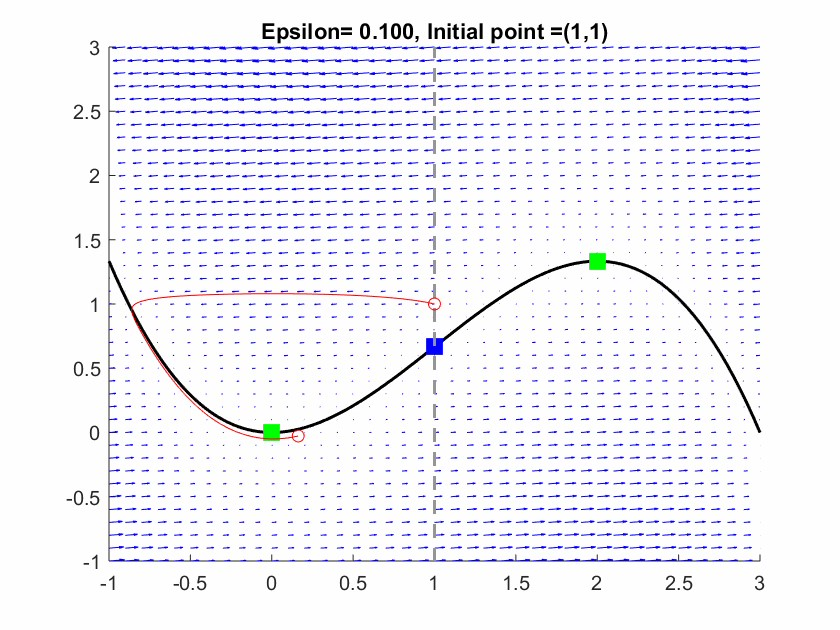
\includegraphics[width=.8\linewidth]{vdPhopf-Moment-3.jpg}
		\caption{The flow as it intersects with the fold point.} \label{fig:timing3}
	\end{subfigure}
	\hfill
	\begin{subfigure}[t]{0.45\textwidth}\centering
		% just an empty subfigure to shift C below A
		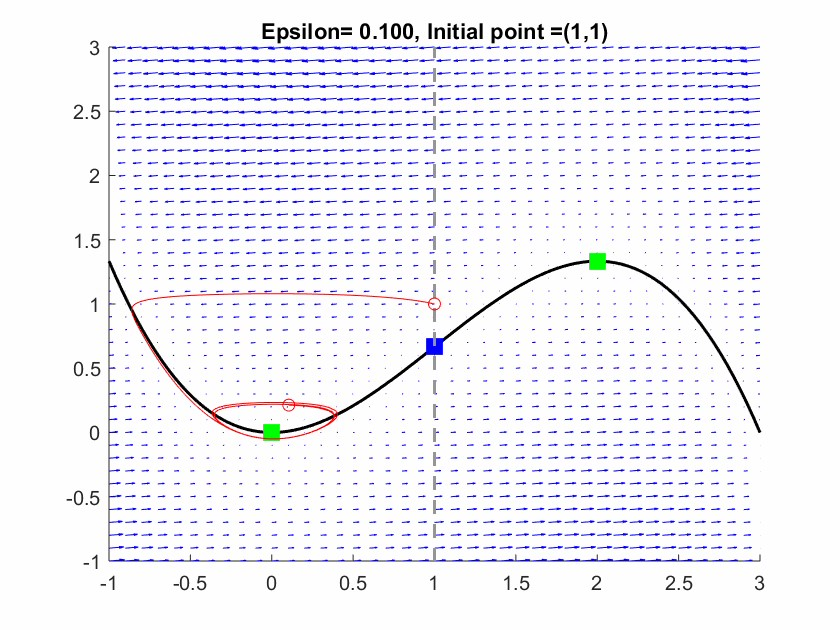
\includegraphics[width=.8\linewidth]{vdPhopf-Moment-4.jpg}
		\caption{The Hopf bifurcation due to the canard point.}\label{fig:timing4}
	\end{subfigure}\vspace{1cm}
	\begin{subfigure}[t]{0.45\textwidth}\centering
		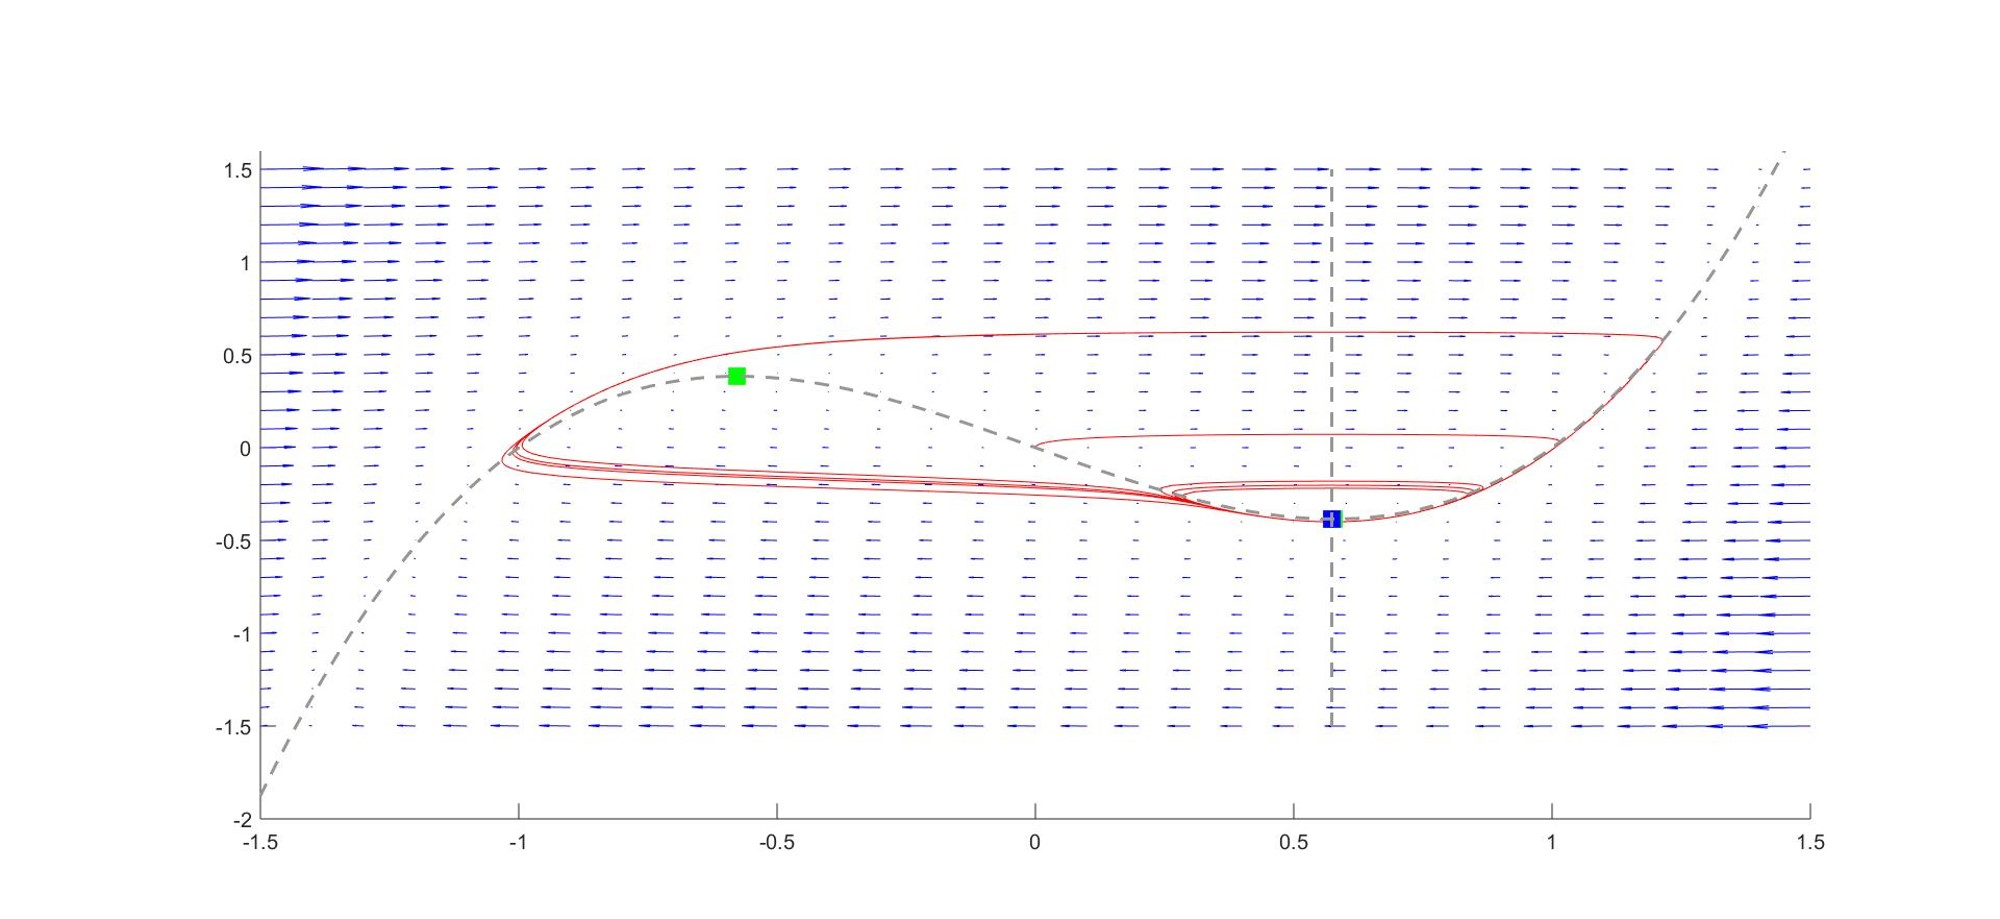
\includegraphics[width=.8\linewidth, height=6cm]{Code/behaviourswitch-pres}
		\caption{Growth of the Hopf bifrucation leading to the formation of a Canard explosion.}
		\label{fig: hopf growth}
	\end{subfigure}
	\caption{The trajectories associated with the canards case of the \vdp system.}
	\label{fig: 4 canard }
\end{figure}\newpage
From Figure \ref{fig: 4 canard } we can see the progression of our flow over the system. From Figure \ref{fig:timing1} we see that the flow starts at an initial condition of $ (x,y)=(1,1) $ and travels along the fast flow towards the attracting branch. Then from Figure \ref{fig:timing2} the flow has hit the attracting branch, where it then follows along the slow flow towards the fold point at $ (x,y)=(0,0) $, which is described by Figure \ref{fig:timing3}. Then from Figures \ref{fig:timing3} and \ref{fig:timing4} we can observe the Hopf bifurcation. This is because we make note that the canard point is present at $ -\lambda $, which in essence pushes the flow up the repelling branch (see Figure \ref{fig: Canard Point}) until the flow is sufficiently far from the fold point where it will then repel towards the attracting branch, starting the growing oscillations - Figure \ref{fig:timing4}. When the Hopf bifurcation is large we would then expect to see a jump in our solution to an attracting branch - Figure \ref{fig: hopf growth}.

%\begin{figure}[h!]\centering
%	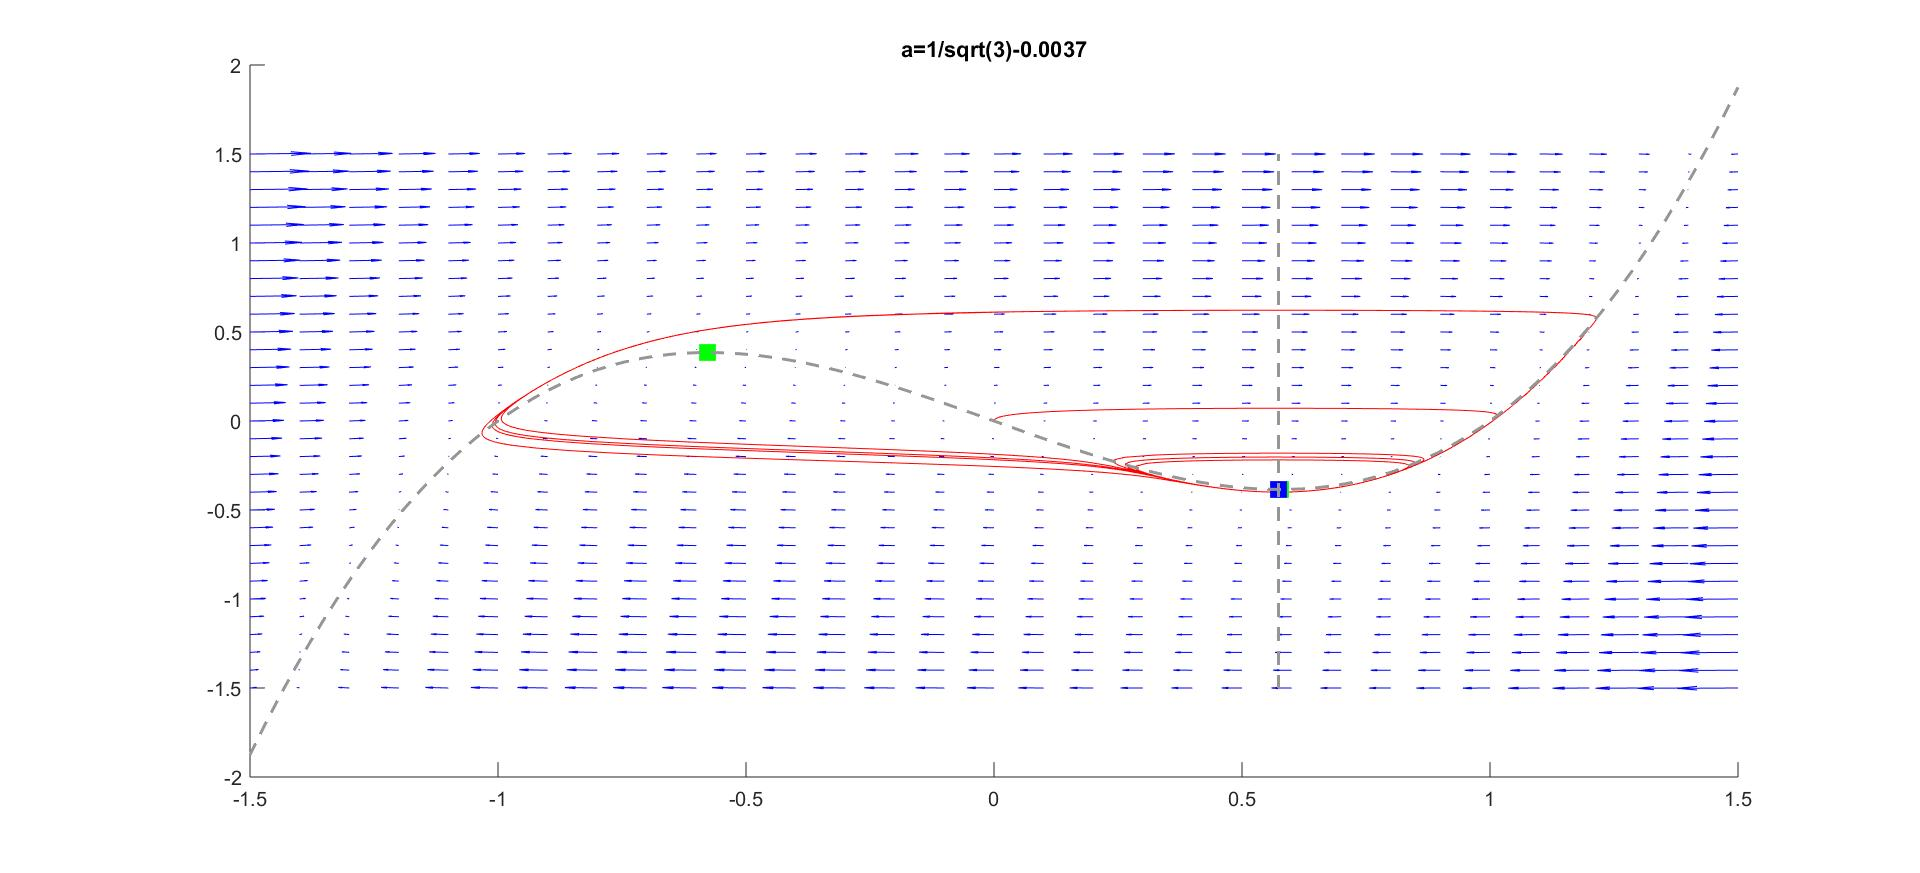
\includegraphics[height=8cm,width=6cm]{Code/behaviourswitch}
%	\caption{Growth of the Hopf bifrucation leading to the formation of a Canard explosion.}
%	\label{fig: hopf growth}
%\end{figure}\newpage
%
%Moreover, it is worth noting that our Hopf bifurcation only exists when we are in an arbitrarily small region, $ O(\epsilon) $, due to the local nature of the theorem \cite{Eckhaus}. 
%\begin{figure}[h!]\centering
%%	\includegraphics[]{}
%	\caption{Development of the Hopf Bifurcation. \textbf{Tom can you screenshot the flow in 4 places?}}
%	\label{fig: Hopf}
%\end{figure}
%Figure \ref{fig: 4 canard } shows that we have an unstable periodic solution within our canard system. In addition to this we know that our canard system will only exist within a small region of $ O(\epsilon) $ \citep{Eckhaus}. Moreover, we can see from Figure \ref{fig: Hopf} that our flow follows the expected path, as we saw in ++++++++++++++++++++++++\\
%%%%%%%%%%%%%%%%%%%%%%%%%%%%%%%%%%%%%%%%%%%%%%%%%%%%%%%%%%%%%%%%%%%%%%%%%%%%%%%%%%%%%%%%%%%%%%%%%%%%%%%%%%%%%%%%%%%%%%%%%%%%%%%%%%%%%%%%%%%%%%%%%%%%%%%%%%%%%%%%%%%%%%%%%%%%%%
%\subsubsection{Singular Hopf Bifurcation}\label{sec:singular-hopf-bifurcation}
%Furthermore, in the \vdp we are able to find a singular Hopf Bifurcation when $ \lambda=1 $. Then to model this behaviour we need to consider a small perturbation along the slow flow where we will have, from Equation \ref{eq: canard system},%discuss what the solutions for x is in the paper 
%\begin{equation}
%\dot{y}=\lambda-x+\bar{\nu} y,
%\end{equation}
%where $ \nu $ is of order $ O(\epsilon) $, thus small. We can immediately see that when $ \bar{\nu}=0 $ that we have our original flow at our equilibrium but we are now able to perturb our flow over a small domain, which are described in Figures \ref{fig: Hopf}. We can also see how our system behaves when our $ \nu $ is of larger order than $ O(\epsilon) $,
%
%\begin{figure}[h]\centering
%	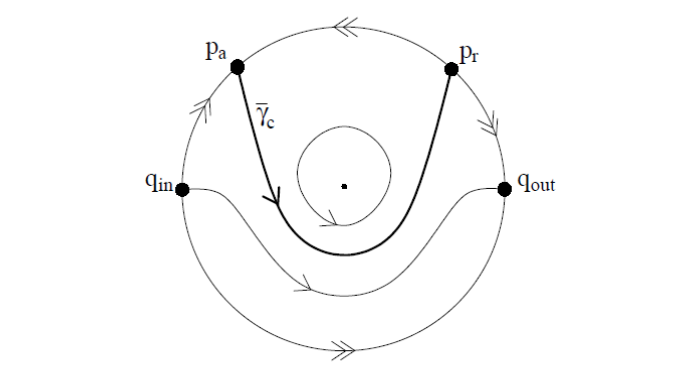
\includegraphics[height=6cm,width=10cm]{Images/CanardPointcircle}
%	\caption{The flow within our canard system \citep{krupa2001}.}
%	\label{fig: canard flow circle}
%\end{figure}\newpage
%where it is clear that our Hopf bifurcation is the periodic solution in the centre of Figure \ref{fig: canard flow circle} but we can see that below our special flow $ \bar{\gamma_c} $ (for the flow outside of the domain $ O(\epsilon) $),our solution traverses through our equilbrium into our fast flow as we would expect in our original system.

%%%%%%%%%%%%%%%%%%%%%%%%%%%%%%%%%%%%%%%%%%%%%%%%%%%%%%%%%%%%%%%%%%%%%%%%%%%%%%%%%%%%%%%%%%%%%%%%%%%%%%%%%%%%%%%%%%%%%%%%%%%%%%%%%%%%%%%%%%%%%%%%%%%%%%%%%%%%%%%%%%%%%%%%%%%%%%

%\subsubsection{Singular Hopf Bifurcation}\textbf{Does this section tie in anywhere else?}
%In this section we will further expand on our Hopf Bifurcation of the previous section (Section \ref{sec:effect-of-the-canard-point}). We note that we get a singular bifurcation iff our system is equivalent to Equation \ref{eq: Fast System}, \st $ \lambda=1 $. \citet{Eckhaus} discusses that our bifuraction will only exist within a small range of $ O(\epsilon) $. Then to model this behaviour we need to consider a small perturbation along the slow flow where we will have, from Equation \ref{eq: canard system},%discuss what the solutions for x is in the paper 
%\begin{equation}
%\dot{y}=\lambda-x+\bar{\nu} y,
%\end{equation}
%where $ \nu $ is of order $ O(\epsilon) $, thus small. We can immediately see that when $ \bar{\nu}=0 $ that we have our orignal flow at our equilbrium but we are now able to perturb our flow over a small domain, which are described in Figures \ref{fig: Hopf}. We can also see how our system behaves when our $ \nu $ is of larger order than $ O(\epsilon) $,
%
%\begin{figure}[h]\centering
%	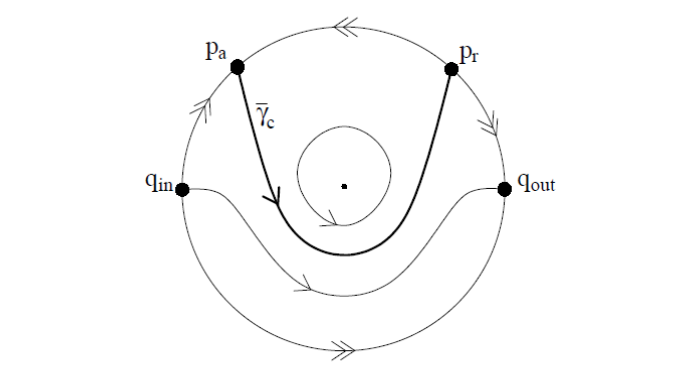
\includegraphics[height=6cm,width=10cm]{Images/CanardPointcircle}
%	\caption{The flow within our canard system \citep{krupa2001}.}
%	\label{fig: canard flow circle}
%\end{figure}\newpage
%where it is clear that our Hopf bifurcation is the periodic solution in the centre of Figure \ref{fig: canard flow circle} but we can see that below our special flow $ \bar{\gamma_c} $, our solution traverses through our equilbrium into our fast flow as we would expect in our original system.

%\newpage


\subsubsection{Separation of the Manifolds}\label{sec:separation-of-the-manifolds}
\begin{figure}[h!]\centering
	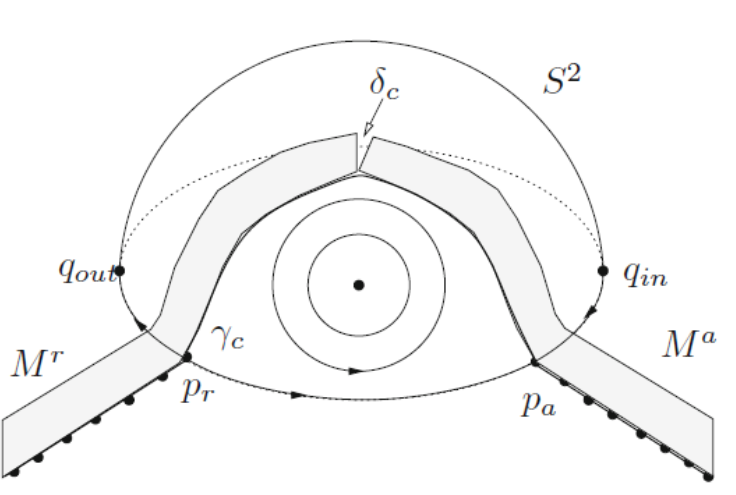
\includegraphics[height=8cm,width=10cm]{Images/Separation}
	\caption{Separation of $ M_a $ and $ M_r $ \citep{Kuehn}.}
	\label{fig: splitting}
\end{figure}%\newpage
%\textbf{Discuss splitting on the manifold}
Continuing on from the singular Hopf bifurcation we might find that the canard point forces our branches to split. In other words we are looking for when the attracting and repelling branches are no longer connected, as show in Figure \ref{fig: splitting}. To do this we would use Melnikov Computations to show that our manifolds split - see \textit{Extending Geometric Singular Perturbation Theory to Nonhyperbolic Points - Fold and Canard Points in Two Dimensions} \citep{krupa2001} for direct use. To discover whether we have a splitting between our branches we need to consider our $ y $ coordinates \wrt our second chart \st $ y_{a,2}(0)-y_{r,2}(0) $ is a distance function which can be written as $ D_c(r_2,\lambda_2)=H(0,y_{a,2}(0))-H(0,y_{r,2}(0)) $ as we note that $ \pd{}{y_2}H(0,y_2)\neq 0 $ \citep{krupa2001}. From here we can use the following proposition,
\begin{prop}
	[\citealp{krupa2001}]
	For a small enough $ \rho $ and $ \mu $ the distance function has the expansion
	\begin{equation*}
	D_c(r_2,\lambda_2)=d_{r_2}r_2+d_{\lambda_2}\lambda_2+O(2),
	\end{equation*}
	where we have defined,
	\begin{subequations}
		\begin{align}
		d_{r_2}&=\int_{-\infty}^{\infty}\text{grad}H(\gamma_{c,2}(t))^T\cdot G(\gamma_{c,2}(t))dt,\\
		d_{\lambda_2}&=\int_{-\infty}^{\infty}\text{grad}H(\gamma_{c,2}(t))^T\cdot (0,-1)^T,
		\end{align}
	\end{subequations}
	and our matrix $ G(\gamma_{c,2}(t)) $ in Section \ref{sec:dynamics-in-texorpdfstringk1k1} with $ \gamma_{c,2} $ as our critical trajectory. 
\end{prop}
Then, following the proof provided by \citet{krupa2001}, we find that we will have a split occurring between our branches if the canard falls outside of our domain of order $ O(e^{-\frac{c}{\epsilon}}) $ \st $ D_c(r_2,\lambda_2)\neq 0 $. We can calculate this explicitly for the the \vdp system by using Equations \ref{eq: const of motion}, \ref{eq: gamma c2} and $ G(x_2,y_2)=(-\frac{x_2^3}{3},0)^T $ \st we have,
\begin{subequations}
	\begin{align}
		d_{r_2}&=\int_{-\infty}^{\infty} \nabla\left(\frac{1}{2}e^{-2y_2}\left(y_2-x^2_2+\frac{1}{2}\right)\right)^T\cdot\left((-\frac{x_2^3}{3},0)^T\right)|_{\gamma_{c,2}} \text{dt}\\
%	&=\int_{-\infty}^{\infty}\left(-\frac{\exp\left(-\frac{t^2}{2}+1\right)}{2}.\frac{\exp\left(-\frac{t^2}{2}+1\right)}{2}\left(\frac{t^2}{4}-\frac{1}{2}-\frac{t}{2}\right)\right)
		&=
	\end{align}
\end{subequations}


 As a result of we see a flow similar to Figure \ref{fig: splitting} whereby we find that our flow could either jump off under the fast flow - see Figure \ref{fig: vdp flow diagram e} - or we might find that the flow could be trapped in the canard region and then be repelled back to the attracting manifold, as we see with our connected system - Figure \ref{fig: 4 canard }. 

\textbf{Good to have a figure if possible}






\section{Folded Singularities in a Three Dimensional System}

%\section{Folded Singularities in three dimensions}
Now that we have considered the two dimensional case for a folded singularity we can extend it to a third dimension in our system. This can be done by considering a system of one fast and two slow variables \st, 
\begin{equation}
\begin{cases}
\epsilon \dot{x}&=f(x,y,z,y,\epsilon),\\
\dot{y}&=g_1(x,y,z,y,\epsilon),\\
\dot{z}&=g_2(x,y,z,y,\epsilon),
\end{cases}
\end{equation}
which we can see is an extension of our original form - Equation \ref{SlowS} \citep{MMO}. Furthermore, \citet{MMO} also discusses that the addition of an extra slow variable causes issues with respect to the existence of a canard solution. This is because our existence ranges increases from $ O(\epsilon) $ to $ O(1) $, noting that $ \epsilon\ll 1 $ \citep{MMO}. Then for this system we are able to make similar assumptions to the previous case, Section \ref{sec:singularities-and-fold-points}, but it is obvious we now must have more than one fold point. We can see that this is the case in Figure \ref{fig: 3d folded singularity},
\begin{figure}[h!]\centering
	%	\includegraphics{}
	\caption{Three dimensional folded singularity.}
	\label{fig: 3d folded singularity}
\end{figure}
as our fold point now can take multiple locations within our system. From here we are able to define some non-degeneracy conditions, much like we did in Section \ref{intro},
\begin{equation}
\begin{aligned}
&f(p_*,\lambda,0)=0,\\
&\pd{}{x}f(p_*,\lambda,0)=0,\\
&\pd{^2}{x^2}f(p_*,\lambda,0)\neq 0,\\
&D_{(y,z)}f(p_*,\lambda,0) \ \text{has full rank one},
\end{aligned}
\label{eq: non-degeneracy 3d system}	
\end{equation}
where we denote $ p_*=(x_*,y_*,z_*)\in F $ as our fold points and $ D_{(y,z)} $ as our Jacobian \wrt $ y \ \text{and}\ z $ \citep{MMO}. In addition to this we can see from Figure \ref{fig: 3d folded singularity} that we have some interesting flows within our system. These flows do not follow the standard pattern as we saw in Figure \ref{fig: vdp flow diagram}, instead the slow flow switches its orientation when the flow hits the fold point and continue to flow in that direction, as a desingularised flow - these are called isolated singularities \citep{MMO}. %dot in diagram
As a result we are able to express these flows in the following manner, using Equation \ref{eq: non-degeneracy 3d system}, 
\begin{equation}
\begin{cases}
\dot{x}&=g_1\pd{f}{y}+g_2\pd{f}{z}\\
\dot{y}&=-g_1\pd{f}{x},\\
\dot{z}&=-g_2\pd{f}{x},
\end{cases}
\end{equation}
where we can then define a folded singularity if $ g_1(p_*,\lambda,0)\pd{}{y}f(p_*,\lambda,0)+g_2(p_*,\lambda,0)\pd{}{z}f(p_*,\lambda,0)=0 $, for our flow on branches ($ S $) \citep{MMO}. Next we need to consider the stability of our fold points. We do this by constructing the Jacobian of our system, 
\begin{equation}
J=\begin{bmatrix}
\pd{\dot{x}}{x}&\pd{\dot{x}}{y}&\pd{\dot{x}}{z}&\pd{\dot{x}}{\lambda}&\pd{\dot{x}}{\epsilon}\\
\pd{\dot{y}}{x}&\pd{\dot{y}}{y}&\pd{\dot{y}}{z}&\pd{\dot{y}}{\lambda}&\pd{\dot{y}}{\epsilon}\\
\pd{\dot{z}}{x}&\pd{\dot{z}}{y}&\pd{\dot{z}}{z}&\pd{\dot{z}}{\lambda}&\pd{\dot{z}}{\epsilon}\\
\end{bmatrix},
\end{equation}
which we can easily find the eigenvalues, by taking the determinant. The result of this analysis gives that we have three eigenvalues, $ \sigma_i $ for $ i=1,2,3 $ \citep{MMO}. \Wlg we can choose $ \sigma_3=0 $ because we know that at least one of our eigenvalues must be zero to account for our fold point in our system, as the \textbf{Poincar\'e diagram describes}. Then we know from standard stability theory that, at our folded singularity we will have three types of phase portrait in the form of,
\begin{equation}
\begin{cases}
Saddle \ \sigma_1\sigma_2<0: \sigma_i\in\Re,\\
Node \ \sigma_1\sigma_2>0: \sigma_i\in\Re,\\
Focus \ \sigma_1\sigma_2>0: \Im(\sigma_i)\neq 0,
\end{cases}
\end{equation}
where we can note that only our focus will have imaginary parts \citep{MMO}. \citet{MMO} illustrates this in the following Figure, 
\begin{figure}[h!]\centering
	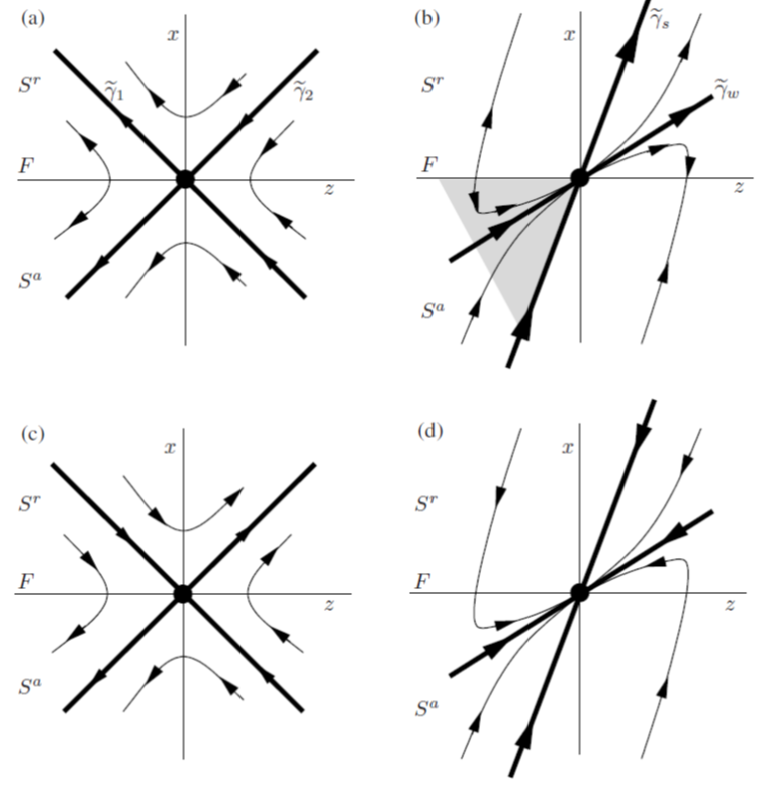
\includegraphics[height=12cm,width=12cm]{Images/foldednodesetc}
	\caption{Phase portraits of our three dimensional system where a) is a folded saddle, b) folded node, c) and d) are desingularised flows \citep{MMO}.}
	\label{fig: folded singularities}
\end{figure}
where we can see the effect of the varying eigenvalues above. A question which is prudent to consider is, why hasn't \citep{MMO} illustrated the singular canard case for a folded focus. This is easily answered as we know that a singular canard is only present if the node or saddle connect our two connecting branches ($ S^r $ and $ S^a $) whereas we find that for the focus \textbf{this is not the case due to its imaginary parts?} \citep{MMO}. This then leads us to the idea of a maximal canard where by only singular canrards can be candidates for these \citep{MMO}. From this \citet{MMO} discusses the following theorem.
\begin{theorem}[Canards in $ \Re^3 $]
	stuff
\end{theorem}



\section{MMO}
\subsection{Oscillations}\label{sec: MMO Oscilaltions} %Need this to reference the oscilatory behavious of the system
In this section we consider Mixed Mode Oscillations (MMOs) in fast-slow systems.++Motivation for studying these+++
++++ add that we consider the work from the \citet{MMO} paper unless indicated otherwise

\begin{definition}{Mixed Mode Oscillations}[\citealp{kuehn}][\citealp{MMO}]
	A mixed mode oscillation is an orbit $\gamma$, which traces out small amplitude oscillations (SAOs) as well as large amplitude oscillations (LAOs).
	The SAOs and LAOs are clearly separated in the time series and their reoccurence can be periodic.
	The signiture of an MMO is expressed as $L_1^{s_1}L_2^{s_2}...$, indicating that $L$ number of LAOs are followed by $s$ SAOs.
\end{definition}

The cases of MMOs considered here are MMOs associated with folded nodes as well as folded saddle-nodes of type 2, that are associated to singular hopf bifurcations.
+++++++++++needs better intro.++++++++++++

\subsection{ Folded Nodes}
In this section the occurence of different SAOs due to a folded node of the reduced system is discussed and conditions for a global return mechanism, which gives rise to MMOs, are presented.
The folded node singularity is an equilibrium of the reduced system. Note that it is only defined on $S$, the critical manifold and therefore only for the slow flow. There is no global equilibrium, wich will become apparent in this section.
The normal form considered for analysing the folded node singularity is in terms of the space variables $(u,v,w)$, and given by:

\begin{align*}
\epsilon \dot{u} &= v - u^2\\
\dot{v} &= w-u\\
\dot{w} &= - \nu
\end{align*}

Then the system can be transformed using the following coordinate and time transformation:
\begin{align}\label{normalform1}
u= \frac{x}{(1+ \mu)^{1/2}}, \ \ \ v &= \frac{y}{(1 + \mu)}, \ \ \  w= -\frac{z}{ (1+\mu)^{3/2}}  \\
\tau &= \frac{\tau_1}{\sqrt{1 + \mu}},
\end{align}
where $\tau_1$ is the original time variable and $\tau$ is the transformed time variable.
Then $\frac{d \tau}{d \tau_1} = \frac{1}{\sqrt{1+ \mu}}$, and the system becomes:
\begin{align}\label{normalform2}
\epsilon \dot{x} &= y - x^2\\
\dot{y} &=- z -(\mu +1)x \\
\dot{z} &= \nu (1 + \mu)^2
\end{align}
where $\mu$ is the eigenvalue ratio from before.
This is nearly in the form presented in \citet{MMO}, however, the $z$ equation there is witten purely in terms of $\mu$ as $\dot{z} = \frac{1}{2} \mu$.
Equating these two representations yields a relationship between $\mu$ and $\nu$:
\begin{align*}
&\nu (1 + \mu)^2 = \frac{1}{2} \mu \\
&\Rightarrow \nu = \frac{\mu}{ 2 (1+ \mu)^2},
\end{align*}
and this is equivalent to 
\begin{align*}
\mu = \frac{ -1 + \sqrt{1 - 8\nu}}{-1 - \sqrt{ 1- 8 \nu}},
\end{align*}
since $0< \mu < 1$ and $\mu \in \mathbf{R}$. (++++ unsure about reasoning+++)

Note here that the reason that no global equilibrium exists is because \ref{normalform1} can only have an equilibrium if $\dot{w} =0$. This would imply that $\nu=0$, however, as the previous calculations have shown, $\nu$ is dependent on the eigenvalue ratio $\mu$. Since $\mu \neq 0$ for the folded node, as will be demonstrated below, $\nu$ cannot be zero.
It is now of interest to verify the location of the folded singularity at the origin, and therefore derive the reduced system as well as the eigenvalues for the reduced problem.
Consider equation (\ref{normalform2}) and define $\dot{x}:=f$ as before. The reduced problem, as $\epsilon \to 0$ becomes $f= y-x^2 =0$, and therefore the critical manifold is defined as $S:= \{ (x,y,z) : y=x^2\}$, which is an S shaped two dimensional plane.
Now that $f$ is defined explicitly, we can check the nondeceneracy conditions for a folded singularity, as presented in (\ref{eq: non-degeneracy 3d system}) and get the follwing results:
\begin{align*}
&f(x,y,z,,\mu, \epsilon) = 0\\
&\Rightarrow y=x^2\\
\\
&\frac{\partial f}{\partial x} (x,y,z,\mu,\epsilon) = 2x = 0\\
&\Rightarrow x=0 \Rightarrow y=0 \\ 
&\frac{\partial^2 f}{\partial x^2}(x,y,z,\mu,\epsilon)  = 2 \neq 0\\
&D_{(y,z)}f= (1,0) \textrm{ full rank one}.
\end{align*}
This shows that there exists a fold line $L:=(0,0,z)$ on the slow manifold $S$.
In order to determine at which value of $z$ the folded node singularity is located, we have to consider the reduced system of (\ref{normalform2}), where we replace $\nu (1 + \mu)^2$ with $\frac{1}{2} \mu$ for convenience. The aim is to find an equilibrium of the reduced problem, since we know from the theory discussed that the folded singularity is an equilibrium of the slow flow.
The reduced problem is:
\begin{align}\label{normalform2red}
0 &= y - x^2 :=f\\
\dot{y} &=- z -(\mu +1)x \\
\dot{z} &=\frac{1}{2} \mu 
\end{align}
Therefore, the slow flow is derived, analogous to Section (I+++ i guess VDP but also after that+++). 
First, the equation $f=0$ is considered and it is noted that we can take the derivative with respect to the time variable to get 
\begin{align} \label{yxderivrel}
\dot{y} = 2x \dot{x},
\end{align}
 and this can be rearranged to give an expression for the dynamics in $x$ on the slow manifold:
\begin{align*}
\dot{x}= \frac{\dot{y}}{2x},
\end{align*}
which is singular for $x=0$, which coinsides with the fold line.
This expression can be desingularised by rescaling time in the whole reduced system by a factor of $2x$. This results in
\begin{align} \label{fullredsysformmo}
&\dot{x} = -(\mu+1)x - z \notag \\
&\dot{y} = - 2x (\mu +1) -2xz\\
&\dot{z} = x \mu \notag,
\end{align}
however, it can be noted that the equation for $y$ can be ommited, since the change in $y$ is directly related to the change in $x$ by a factor of $2x$ as stated in equation (\ref{yxderivrel})(+++mention CMT?+++). Therefore, the reduced dynamics can be sufficiently described by
\begin{align}\label{twovarxzred}
&\dot{x} = -(\mu+1)x - z\\
&\dot{z} = x \mu. \notag
\end{align}
Now, following the theory for folded singularities, the folded node has to satisfy the condition (+++add name of the condition and generalized statement of it+++)
\begin{align*}
& -(\mu+1)x - z=0 |_{(0,0,z)}\\
&\Rightarrow z=0,
\end{align*}
which leads to the conclusion that the folded singularity, defined on the slow manifold for $\epsilon \to 0$ and located on the fold line $L=(0,0,z)$, is given by $(0,0,0)$, as expected.
The next step of the analysis is to verify that the folded singularity at the origin is indeed a folded node.
As discussed in Section \ref{sec: threedimfolds}, the classification of the singularities is determined by the eigenvalues of the reduced system. Therefore, the next step is calculating these eigenvalues.
The Jacobian of the reduced system (\ref{twovarxzred}) is
\begin{equation}
J=\begin{bmatrix}
-(\mu +1) & -1 \\
\mu & 0 \\
\end{bmatrix},
\end{equation}
and therefore the characteristic equation yields
\begin{align*}
&\sigma^2 +(\mu +1)\sigma + \mu = 0 \\
&\Rightarrow \sigma_1= -1 \textrm{\ \ \ and \ \ \ } \sigma_2 = -\mu.
\end{align*}
Since $\mu$ is the eigenvalue ratio and satisfies $0< \mu < 1$, we can conclude that 
\begin{align*}
\sigma_1\sigma_2 = (-1)(-\mu)=\mu >0,
\end{align*}
and therefore, by the conditions presented in Section \ref{sec: threedimfolds}, this shows that the folded singularity is in fact a folded node.
Note that if we had tried to find the eigenvalues for the full three dimensional reduced system (\ref{fullredsysformmo}) instead, an additional eigenvalue $\sigma_3=0$ would have occured. This is the eigenvalue that corresponds to the loss of hyperbolicity at the folded node, which is expected for singular points.

In order to analyse the folded node, the system (\ref{normalform1}) is transformed using the blow up transformation $u= \epsilon^{1/2}\overline{x}, v=\epsilon \overline{y}, w= \epsilon^{1/2} \overline{z}$ and $ \tau_1 = \epsilon^{1/2} \overline{t}$.
Then, in a neighbourhood $U$ of the folded node the system is represented by
\begin{align*}
\dot{\overline{x}}= \overline{y} - \overline{x}^2\\
\dot{\overline{y}}=\overline{z} - \overline{x} \\
\dot{\overline{z}}= - \nu.
\end{align*}
In the following analysis, the bars will be omitted for readability.
One important realisation is that the phase portraits for the rescaled system is topologically equivalent to the original normal form. Therefore, the mapping of solutions  found in the blown up system to the original system is straightforward. ++++check if true++++

All the information needed to describe the dynamics near the fold point is now derived and therefore the next step in the analysis is the descripton of the SAOs. The SAOs in the folded node case are candard trajectories that follow a certain pattern.
These patterns are, as discussed in Theorem \ref{thm: canards in R3}, found by considering the eigenvalue ratio $\mu$.
In the case of the folded node, $\mu$ satisfies $2k+1 < \mu^{-1} < 2k +3 $. Solving for $k \in \mathbf{N}$, then $k$ is the number of secondary canards in the system as stated in Theorem \ref{thm: canards in R3}. Furthermore, $k$ corresponds to the number of twists the primary canard $\gamma_s$ is performing around $\gamma_w$. A twist corresponds to a $180^{\circ}$ rotation, see \citet{kuehn}. It is important to note that $\mu^{-1} \notin \mathbf{N}$ in order to conclude the number of secondary canards.
If $\mu^{-1} \in \mathbf{N}$ 

These SAOs are happening when trajectories get funneled into the region of the fold and contracted along the direction of $S^a$(+++++?????++++). For different values of $\epsilon$, the funnel gets narrower. For $\epsilon \to 0$, the maximum canard basically coinsides with all of them... or something like that....
The number of SAOs an incoming trajectory undergoes depends on where the trajectory enters the fold region in the $z$ plane. Different intervals of $z$ can be defined in order to indicate for which values of $z$ a certain amount of SAOs will be observed. The intervals are not 'clear cut', and a mix can happen +++??+++
The interval for the primary strong canard is significantly larger, so the secondary canards close to it will have a higher amplitude (? reasoning right?) while the number of SAOs is smaller. As the number of SAOs increases, the amplitude of oscillations get smaller (contraction ?) and are not readily visible.
The result about the width of the intervals is summed up in the following theorem.

\begin{theorem}[\textbf{Width of Rotational Sectors} \citealp{MMO}]
Consider system (\ref{somegenericthreedim}) and assume it has a folded-node singularity. At an $O(1)$ distance from the fold curve, all secondary canards are in an $O(\epsilon^{(1- \mu)/2)})$ neighbourhood of the primary strong canard. Hence, the width of the  rotational sectors $I_i, 1 \leq i \leq k$, is $O(\epsilon^{(1- \mu)/2)})$ and the width of sector $I_{k+1}$ is $O(1)$.
\end{theorem}

++++++++++Maybe the actual pictures (2-3) would be a good idea++++++ 

+++++++++++Return Mechanism++++++
As mentioned above, there are certain criteria that indicate the existence of a global return mechanism and therefore that MMOs can be observed.
There are two theorems related to this issue, which are stated below.
The first one is rather technical, stating the existence of the global return under certain circumstances, when the trajectory is in the rotational sector $I_{k+1}$, meaning, close to the weak primary canard and the $k+1$ number of SAOs, is hard to observe. Furthermore, as mentioned above, the width of the sector is much smaller than that of the primary canard, which is why the oscillations happen with fast speed, Therefore, the logical conclusion is to investigate whether a global return mechanism exists for the other $I_i$, for $i \leq k$. The existence of these MMOs is discussed in the second Theorem in this section.
As introduced in the beginning of Section \ref{sec:MMO},  the signatures of MMOs are represented in terms of the number of large amplitude oscillations $L_1L_2...$ and the number of small amplitude oscillatons $s^1s^2...$, and the conventional notation is $L_1^{s^1}L_2^{s^2}....$.
In the case of the folded node, under the conditions of the theorems, we have a rather straightforward signature. The first theorem states the existence of the signature $1^{k+1}$, where $L_1=1$ and $s^1=k+1$, and equivalently, the second theorem in this chapter discusses MMOs with signature $1^{i}, i<k$.
The theorems are as follows.
(++ $K+1$ are maximal MMO signatures++++) something about deltas too++++
\begin{theorem}[\textbf{Generic $1^{k+1}$ MMOs}][\citealp{MMO}] \label{MMOsigk1}
Consider system (\ref{somegenericthreedim}) with the following assumptions:
\begin{enumerate}
\item Assume that $ 0 < \epsilon \ll 1$ is sufficiently small, $\epsilon^{1/2} \ll \mu$, and $k \in \mathbf{N}$ is such that $2k + 1 < \mu^{-1} < 2k + 3$.
\item The critical manifold $S$ is (locally) a folded surface.
\item The corresponding reduced problem possesses a folded-node singularity.
\item There exists a candidate periodic orbit, which consists of fast fibres of the layer problem, a global return segment, and a segment on $S^a$ within the funnel that starts at distance $\delta$ from $\overline{\gamma_s}$ ( as measured at a distance $O(1)$ away from the fold $F$).
\item An appropriate transversality hypotheses is satisfied.
\end{enumerate}
Then there exists a stable MMO with signature $1^{k+1}$.
\end{theorem}

\begin{theorem}[\textbf{Stable MMOs with signature $1^i$} \citealp{MMO}]
Suppose system (\ref{somegenericthreedim}) satisfies assumptions 1. - 4. of Theorem \ref{MMOsigk1} and, the following additional assumption:
\begin{itemize}
\item For $\delta = 0$, the global return point is on the singular strong canard $\overline{\gamma_s}$ and as $\delta$ passes through zero the return point crosses $\overline{\gamma_s}$ with nonzero speed.
\end{itemize}
Suppose now that $\delta= O(\epsilon ^{(1-\mu)/2})>0$. Then, for sufficiently small $0 < \epsilon \ll 1$ and $k \in \mathbf{N}$ such that $2k+1 < \mu^{-1} < 2k+ 3$, the following holds.
For each $i, 1 \leq i \leq k$, there exist subsectors $\overline{I}_i \subset I_i$ with the corresponding distance intervals $(\delta_i^-, \delta_i^+)$ of widths $O(\epsilon^{(1-\mu)/2})$, which have the property that if $\delta \in (\delta_i^-, \delta_i^+)$, then there exists a stable MMO with signature $1^i$.
\end{theorem}

+++++++i think more talk about funnels and contractions would be good for this chapter+++++++++
all we need is the trajectory to go back into the funnel region. then we're good :)


















































\subsection{Singular Hopf Bifurcation}
In this section the folded saddle-node of type 2 and the saddle focus are considered for analysis.
The folded saddle-node o type 2 occurs, when the parameters of the system coinside in such a way that an equilibrium of the full system and a fold point coinside. A saddle-node of type one refers to the case when only an equilibrium of the reduced system crosses a fold, without coinciding with a global equilibrium.
If a saddle-node type 2 occurs for a specific parameter (also plural...), then a singular hopf bifurcation arises at $O(\epsilon)$ away from the equilibrium.
The equilibrium is focus if the eigenvalues corresponding to it are complex and a node if the eigenvalues are real.

\begin{definition}{\textbf{Singular Hopf Bifurcation} \citealp{strogatz2007nonlinear}}\\
A singular hopf bifurcation occurs at a certain parameter regime in the system which is $O(\epsilon)$ away from a saddle-node of type 2. There, the eigenvalues of the system cross the imaginary axis, therefore they have a zero real part. Then small oscillations, called limit cycles occur in the system. There are two types of singular Hopf Bifurcation.
The supercritical Hopf Bifurcation occurs when a stable limit cycle arises from an unstable equilibrium point, while the subcritical Hopf Bifurcation causes unstable limit cycles to appear around a stable equilibrium.
\end{definition}

These different orbits caused by a singular Hopf Bifurcation are of interest, because they are SAOs of the fast-slow system in question. Therefore, in this chapter we will give an overview of the different SAOs arising from singular Hopf Bifurcations in different parameter regimes.
The starting point of the analysis is the normal form considered for the folded node in section +++toms section+++, which is then modified to a system that displays a singular Hopf Bifurcation and later on a system with a global return mechanism will be derived.
The first transformation is achieved by adding higher-order terms to the $z$ equation of system (++ toms normal form+++). It then becomes
\begin{align*}
\epsilon \dot{x} &= y - x^2, \\
\dot{y} &= z - x \\
\dot{z} &= - \nu -ax - by - cz,
\end{align*}
which is the normal form for a singular Hopf Bifurcation.
We then consider a coordinate transformation and time rescaling of the form
\begin{align*}
x = \epsilon^{1/2}\overline{x}, \ \ \ y= \epsilon \overline{y},  \ \ \ z = \epsilon^{1/2} \overline{z},\ \ \  t= \epsilon^{1/2} \overline{t}.
\end{align*}
Then the system becomes
\begin{align} \label{sysepsilonenvir}
\overline{x}' &= \overline{y} - \overline{x}^2, \\
\overline{y}' &= \overline{z} - \overline{x}, \\
\overline{z}' &= - \nu - \epsilon^{1/2} a \overline{x} - \epsilon b \overline{y} - \epsilon^{1/2} c \overline{z}.
\end{align}
This transformation can be seen, somewhat equivalently to Section \ref{sec:transform blowup}, as a consideration of a small neighbourhood of the singular point.
As described in Section \ref{sec: threedimfolds}, folded singularity is found by examining the critical manifold $C= \{ (x,y,x) : f:=y-x^2 =0 \}$. The conditions (\ref{eq: non-degeneracy 3d system}) are easily checked and satisfy:
\begin{align*}
f(p_*, \nu, \epsilon)&= y- x^2 =0 \\
\Rightarrow y &= x^2\\
\pd{}{x}f(p_*,\lambda,0) &= -2x = 0,\\
\Rightarrow x &= 0\\
\Rightarrow y &=0\\
\pd{^2}{x^2}f(p_*,\lambda,0) &= -2 \neq 0,\\
D_{(y,z)}f(p_*,\lambda,0) &= (1,0)
\end{align*}
+++++++++++++++++++Help!! Fold conditions do not work out....+ also no idea what the parameters are $\nu, \epsilon$? is it going to zero....+++++++++++++++
The folded singularity is found at $p_*= (0,0,z)$, which makes the further analysis slightly more straightforward.
The equilibria of the system are, such that $p_0= (x,x^2,x)$, where $x$ satisfies:
\begin{align}\label{MMOxsol1}
x = -\frac{1}{2 \epsilon^{1/2} b} \left( (a+c) \pm \sqrt{ (a+c)^2 - 4 b \nu } \right),
\end{align}
and therefore there are two equilibria++++is it correct that i have 2??+++++ at
\begin{align*}
&x_1=-\frac{a+c}{ \epsilon^{1/2} b} + \frac{\nu}{\epsilon^{1/2} (a+c)} + \frac{b \nu^2}{\epsilon^{1/2} (a+c)^3} + ... \\
&x_2= \frac{\nu}{\epsilon^{1/2} (a+c)} + \frac{b \nu^2}{\epsilon^{1/2} (a+c)^3} + ...,
\end{align*}
where a MacLaurin expansion for $\sqrt{ (a+c)^2 - 4 b \nu }$ has been used.
There exists a value for $x$ depending on the parameters $a,b,c$ and $\nu$, where a fold point intersects with the equilibrium. This is at $x_1=0$ and $x_2=0$.
Then, setting (\ref{MMOxsol1}) to zero results in
\begin{align*}
x=-\frac{1}{2 \epsilon^{1/2} b} \left( (a+c) \pm \sqrt{ (a+c)^2 - 4 b \nu } \right)=0\\
\Rightarrow \nu = - \frac{ (a+c)^2 - (a+c)}{4b}.
\end{align*}
Therefore, the location of the singular equilibrium, depends on the parameter values for $a,b,c$.

Since $a, b$ and $c$ are all multiplied by a factor of $\epsilon^{1/2}$ or $\epsilon$ in system (\ref{sysepsilonenvir}), we need $\nu$ to be of $O(\epsilon^{1/2})$ or smaller in order to observe a singular hopf bifurcation.
If $\nu=O(1)$, then the factors of $\epsilon$ in system (\ref{sysepsilonenvir}) do not really contribute to the system and are merely a pertubation of the normal form (++++toms normal form++++).
If $\nu \leq O(\epsilon^{1/2})$, then a singular hopf bifurcation occurs at a distance $\nu =O(\epsilon)$ in parameter space away from the equilibrium.
The eigenvalues of the system (\ref{sysepsilonenvir}) can be found by considering the following Jacobian matrix associated to it:
\begin{equation}
J=\begin{bmatrix}
2x & 1 & 0 \\
-1 & 0 & 1 \\
-\epsilon^{1/2} a & - \epsilon b & - \epsilon^{1/2} c\\
\end{bmatrix}.
\end{equation}
Using a computer package, such as Maple, to solve for the eigenvalues confirms that there exist two complex eigenvalues for the equilibrium where $x=0$.
Since the eigenvalues of the system are complex, the equilibrium is a saddle-focus, which has not been discussed in the analysis of canard trajectories. (+++++loop back to 3dim singularities and why we dont have canards)+++++++
The research of the dynamics, and specifically MMOs, close to a singular Hopf Bifurcation is still ongoing. Here we only consider a few specific cases, where $\nu$ is treated as the main parameter of interest. Furthermore, since the critical manifold in system (\ref{sysepsilonenvir}) is in the shape of a quadratic function, by the geometrical nature of the problem, there is no global return mechanism for the system. Trajectories that leave the close proximity of the equilibrium do not return. In order to get MMOs, additionally to the SAOs a global return mechanism is needed.
This is achieved by modifying system (\ref{sysepsilonenvir}) by adding a cubic term to the $x$ equation. This will change the shape of the critical manifold to an S shaped curve and therefore allow for a global return mechanism. The new system is then the following:
\begin{align*}
\epsilon \dot{x} &= y - x^2 - x^3, \\
\dot{y} &= z - x, \\
\dot{z} &= -\nu -ax -by -cz.
\end{align*}

The expected behaviour of the new system is now to display several SAOs close to the equilibrium, before completing a large amplitude oscillation. This LAO is necessarily of the form of a relaxation oscillation, because there is only one fast variable present in the system. This represents a constraint since the fast subsystem is one dimensional and therefore trajectories are restricted to be monotonic.

There are now many different types of MMOs present, depending on the parameter regimes.
One example is that for small values of $\nu$, where $\nu=O(\epsilon)$, a stable periodic orbit $\Gamma$ arises from the saddle-focus equilibrium. This orbit is tracing out SAOs close tho the repelling sheet of the critical manifold, before completing a relaxation oscillation and returning to its starting point.
However, other bifurcations can occur for these periodic orbits for different parameter regimes. These could be of the form of torus bifurcations or period-doubling. Then there is a possibilities of chaotic MMOs exisiting for these parameters. For decreasing values of $\nu$ here, which is already $O(\epsilon)$, large amplitudes are getting smaller until the system only displays chaotic SAOs(++++++not sure if terminology works like this...+++)

Now it is of interest to consider specific parameter regimes for which the SAOs are constrained to the unstable manifold $W^u(p_*)$, which corresponds to the phase space surrounding the equilibrium $p_*$, while being backward asymptotic to it.
For a supercritical Hopf Bifurcation we just observe the stable oscillation, as before. However, there is another type of bifurcation (+++++WHY+++++++) under certain conditions ($W^u$ tangent tp S)


\newpage 
\bibliography{FastSlow.bib}
\bibliographystyle{agsm}
\nocite{strogatz2007nonlinear}

\newpage
\appendix
\section{Elements of Dynamical Systems}\label{app:DynSys}
In this appendix we state some standard results from dynamical systems theory.
\subsection{Stable Manifold Theorem}
Suppose $\dot{x} = F(x)$ where $x\in \mathbf{R}^n, F\in C^r(\mathbf{R}^n,\mathbf{R}^n)$ and has only hyperbolic fixed points (i.e. in the associated linearised system $\dot{x}=Ax$, $A\in \mathbf{R}^n$ has no eigenvalues $\lambda$ such that $\mathrm{Re}(\lambda)=0$). 
\subsection{Centre Manifold Theorem}
\subsection{Hopf Bifurcations}

\section{Intuitive Examples}\label{sec:definitions}%Defintions not integral to the project
\subsection{Folded Focus}
\label{a: sinksource}
For the folded focus, we will consider an approach from fluid mechanics. This is to enable the reader to consider the dynamics within a different field with the aim to give more intuition in a fast-slow dynamical system. To aid with this concept one should consider the motion of water in a bathtub, when the plug has been removed. We can immediately observe that the water will start to spiral around the plug - much like Figure \ref{fig: spiral} - which acts in a similar fashion to the following figure. 
\begin{figure}[h!]
	\centering
	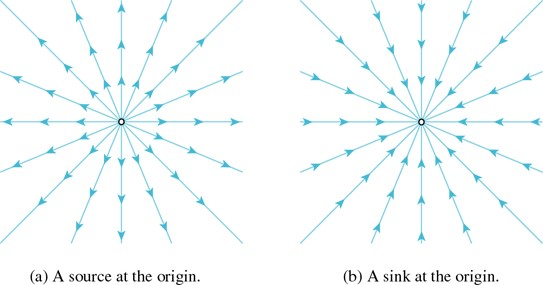
\includegraphics[width=0.7\linewidth]{Images/sourcesink}
	\caption{Oversimplified phase plane for a folded focus.}
	\label{fig:source-sink}
\end{figure}
From Figure \ref{fig:source-sink} we see that on the left we have a source within the system, by this we can observe that a source attracts the flow in the system. Whereas on the right we have a sink which can be seen to be repelling the flow, resulting in the jumps (Figure \ref{fig: vdp flow diagram}) or oscillation in the system - see Sections \ref{sec:singularitiesandfoldpoints} and \ref{sec: MMO Oscilaltions}. 
\section{Numerical Simulation}\label{app:NumSim}

Many figures in this document? were produced using MATLAB, for example: fig +++++++. In this appendix, we will give a brief tutorial on their production. Fast-slow systems like the ones studied here are a classic example of \emph{stiff} ODEs. 
\begin{definition}[Stiffness Ratio]
	Consider $\dot{x} = F(x)$ where $x\in \mathbf{R}^n, F\in C^r(\mathbf{R}^n,\mathbf{R}^n)$. Let 
	$$ z' = Az,\quad A\in \mathbf{R}^{n \times n}  $$
	denote its linearisation. Suppose all the eigenvalues $\lambda_j$  of $A$ have negative real parts. Then the \emph{stiffness ratio}, $\mu$ is defined as
	$$ \mu :=\frac{\max_j(\mathrm{Re}(\lambda_j))}{\min_j(\mathrm{Re}(\lambda_j))} $$
	If $\mu$ is large, the system is called \emph{stiff}.
\end{definition}
If we consider for example the Van der Pol system \ref{eq: Fast System}, its linearisation is
$$ \begin{pmatrix}
x' \\ 
y'
\end{pmatrix}  = \begin{pmatrix}
2x-x^2 & -1 \\ 
\epsilon & 0
\end{pmatrix}  \begin{pmatrix}
x\\y	
\end{pmatrix}  $$
 
\section{Dynamics in \texorpdfstring{$K_2$}{K2}}


\end{document}
